\documentclass[oneside]{book}
\usepackage{titlesec}
\usepackage[inner=2.5cm,outer=2.5cm,top=2.5cm,bottom=2.5cm]{geometry}
\usepackage{ragged2e}
\usepackage[doublespacing]{setspace}
\usepackage{graphicx}
\usepackage[flushleft]{threeparttable} 
\usepackage{fancyhdr, lastpage, bbding, pmboxdraw}
\usepackage[usenames,dvipsnames]{color}
\definecolor{darkblue}{rgb}{0,0,.6}
\definecolor{darkred}{rgb}{.7,0,0}
\definecolor{darkgreen}{rgb}{0,.6,0}
\definecolor{red}{rgb}{.98,0,0}
\usepackage[colorlinks,pagebackref,pdfusetitle,urlcolor=darkblue,citecolor=darkblue,linkcolor=darkred,bookmarksnumbered,plainpages=false]{hyperref}
\renewcommand{\thefootnote}{\fnsymbol{footnote}}

% \pagestyle{fancyplain}
% \fancyhf{}
% \lhead{ \fancyplain{}{BIOL 4020 – Vertebrate Biodiversity - Lab Manual}}
% %\chead{ \fancyplain{}{}}
% \rhead{ \fancyplain{}{Fall 2020}}
% %\rfoot{\fancyplain{}{page \thepage\ of \pageref{LastPage}}}
% \fancyfoot[RO, LE] {page \thepage\ of \pageref{LastPage}}
% \thispagestyle{plain}

%%%%%%%%%%%% LISTING %%%
\usepackage{listings}
\usepackage{caption}
\DeclareCaptionFont{white}{\color{white}}
\DeclareCaptionFormat{listing}{\colorbox{gray}{\parbox{\textwidth}{#1#2#3}}}
\captionsetup[lstlisting]{format=listing,labelfont=white,textfont=white}
\usepackage{verbatim} % used to display code
\usepackage{fancyvrb}
\usepackage{acronym}
\usepackage{amsthm}
\usepackage{arydshln} % dashed line in table
\VerbatimFootnotes % Required, otherwise verbatim does not work in footnotes!



\definecolor{OliveGreen}{cmyk}{0.64,0,0.95,0.40}
\definecolor{CadetBlue}{cmyk}{0.62,0.57,0.23,0}
\definecolor{lightlightgray}{gray}{0.93}



\lstset{
%language=bash,                          % Code langugage
basicstyle=\ttfamily,                   % Code font, Examples: \footnotesize, \ttfamily
keywordstyle=\color{OliveGreen},        % Keywords font ('*' = uppercase)
commentstyle=\color{gray},              % Comments font
numbers=left,                           % Line nums position
numberstyle=\tiny,                      % Line-numbers fonts
stepnumber=1,                           % Step between two line-numbers
numbersep=5pt,                          % How far are line-numbers from code
backgroundcolor=\color{lightlightgray}, % Choose background color
frame=none,                             % A frame around the code
tabsize=2,                              % Default tab size
captionpos=t,                           % Caption-position = bottom
breaklines=true,                        % Automatic line breaking?
breakatwhitespace=false,                % Automatic breaks only at whitespace?
showspaces=false,                       % Dont make spaces visible
showtabs=false,                         % Dont make tabls visible
columns=flexible,                       % Column format
morekeywords={__global__, __device__},  % CUDA specific keywords
}

% No chapter names
\titleformat{\chapter}[display]
  {\normalfont\bfseries}{}{0pt}{\Large}

\usepackage{docmute}
\title{\LARGE{BIOL 4020: Vertebrate Biodiversity}
\author{\Large{Auburn University Lab Manual}
\date{\Large{Fall 2020}}
}}
\begin{document}
\maketitle
\tableofcontents
\chapter{\Huge{Lab Breakdown}} \label{SecLabBreak}
%% LaTeX2e file `LabBreakdown.tex'
%% generated by the `filecontents' environment
%% from source `main' on 2020/08/03.
%%
  \documentclass[11pt, a4paper]{article}
  \begin{document}


\begin{center}
\rule{6in}{0.4pt}
\begin{minipage}[t]{.75\textwidth}
\begin{tabular}{llcccll}
\textbf{GTAs:} & Randy Klabacka: \href{mailto:rlk0015@auburn.edu}{rlk0015@auburn.edu} (702)882-6292 \\ & Morgan Muell: \href{mailto:mrm0161@auburn.edu}{mrm0161@auburn.edu} \\ \textbf{Sections:} & 1: Mon 12:00 -- 2:50 \\ & 2: Tue 12:30 -- 3:15 \\ & 3: Wed 12:00 -- 2:50
\end{tabular}
\end{minipage}
\rule{6in}{0.4pt}
\end{center}
\vspace{.5cm}
\setlength{\unitlength}{1in}
\renewcommand{\arraystretch}{2}

\noindent\textbf{Grade Breakdown:}
\begin{table}[h]
\label{Table:GradeBreakdown}
\begin{tabular}{lll}\hline
Category                     & Points  \\ \hline
Attendance \& Participation  & 20      \\
Project Proposal             & 40      \\
Field Notebook               & 40      \\
Exams (20 pts each, 4 exams) & 80      \\ \hdashline
Total                        & 240     \\ \hline
\end{tabular}
\end{table}

\vskip.15in
\noindent\textbf{Attendance \& Participation:} %\footnotemark
\begin{itemize}
\item{Participation: ~7 points per lab}
\item{Each lab has a corresponding lab module on canvas with instructions on how to obtain points for that lab. Obtaining attendance/participation points for each lab is dependent on completion of the elements within each lab module.}
\item{Each lab module will close at the beginning of the following lab (e.g., the Lab Module for Lab 2 will close once the Lab Module for Lab 3 opens). Lab modules open at the start of lab (i.e., 12:00 pm on Monday for Section 1) and end at the beginning of the following lab (e.g., 11:59 am on the following Monday for Section 1)}.
\item{Failure to attend/participate in a lab results in a loss of all points for that lab.}
\end{itemize}

\vskip.15in
\noindent\textbf{Project Proposal:} %\footnotemark
\begin{itemize}
\item{Rough Draft: 15 points; Final Draft: 25 points}
\item{Additional details for this assignment are on page XXXX}
\end{itemize}

\vskip.15in
\noindent\textbf{Field Notebook:} %\footnotemark
\begin{itemize}
\item{12 hours of in-field observation (including those from lab trips [4 trips: 8 hrs])}
\item{4 points will be deducted for each hour a student is short of the 12 total hours}
\item{Additional details for this assignment are on page XXXX}
\end{itemize}

\vskip.15in
\noindent\textbf{Exams:} %\footnotemark
\begin{itemize}
\item{Exams will be administered electronically over Canvas and will include:}
\begin{enumerate}
\item{Photo identification for focal taxa (common names acceptable)}
\item{Natural history facts discussed in lab/field}
\item{Major points from publications discussed in lab}
\item{Phylogenies for focal taxa}
\end{enumerate}
\end{itemize}


\centering
\begin{table}[h]
\label{Table:Schedule}
\caption{Lab Schedule}
\begin{tabular}{llll}\hline
Week of & Lab Module          & Topic                           & Items due before class  \\ \hline
Aug 17  & Lab 1               & Live zoom overview              &                         \\
Aug 24  & Lab 2               & Intro to Fishes                 &                         \\
Aug 31  & Lab 3               & Field Trip- Euphapee Creek      & Discussion Template     \\
Sep 7   & \textit{No Lab}     & \textit{Labor Day}              &                         \\
Sep 14  & Lab 4               & Intro to Amphibians             & \textbf{Fish Exam}      \\
Sep 21  & Lab 5               & How To Science                  & Proposal Ideas          \\
Sep 28  & Lab 6               & Field Trip- Opacum Pond         & Canvas Discussion       \\
Oct 5   & Lab 7               & Intro to Diapsids               & \textbf{Amphibian Exam} \\
Oct 12  & Lab 8               & Proposal Workshop               & Proposal Rough Draft    \\
Oct 19  & Lab 9               & Field Trip- Wood Duck Preserve  & Discussion Template     \\
Oct 26  & Lab 10              & Intro to Mammals                & \textbf{Diapsid Exam}   \\
Nov 2   & Lab 11              & Field Trip- Oxbow Pond          & Proposal Submission     \\
Nov 9   & Lab 12              & Proposal Panels                 & Proposal Review         \\
Nov 16  & \textit{No Lab}     & \textit{Final Exam Week}        & \textbf{Final Exam}     \\ \hline
\end{tabular}
\bigskip{}
\end{table}


\noindent\textbf{Academic Honesty and Inclusion:}
\begin{itemize}
\item{This lab welcomes, respects, and serves students of diverse backgrounds and perspectives, and it is expected that students respect one another. Any acts of aggression or misconduct based on race, color, religion, age, national origin, sex or sexual orientation, gender identity, or disability will not be tolerated.}
\end{itemize}

  \end{document}
% preamble will be ignored
\chapter{\Huge{Project Proposal}} \label{SecProjProp}
  \documentclass[11pt, a4paper]{article}
  \usepackage[inner=1.5cm,outer=1.5cm,top=2.5cm,bottom=2.5cm]{geometry}

\pagestyle{empty}
\usepackage{graphicx}
\usepackage{setspace}
\usepackage{threeparttable}
\usepackage{fancyhdr, lastpage, bbding, pmboxdraw}
\usepackage[usenames,dvipsnames]{color}
\definecolor{darkblue}{rgb}{0,0,.6}
\definecolor{darkred}{rgb}{.7,0,0}
\definecolor{darkgreen}{rgb}{0,.6,0}
\definecolor{red}{rgb}{.98,0,0}
\usepackage[colorlinks,pagebackref,pdfusetitle,urlcolor=darkblue,citecolor=darkblue,linkcolor=darkred,bookmarksnumbered,plainpages=false]{hyperref}
\renewcommand{\thefootnote}{\fnsymbol{footnote}}

\pagestyle{fancyplain}
\fancyhf{}
\lhead{ \fancyplain{}{Vertebrate Biodiversity Lab- Lab Breakdown} }
%\chead{ \fancyplain{}{} }
\rhead{ \fancyplain{}{\today} }
%\rfoot{\fancyplain{}{page \thepage\ of \pageref{LastPage}}}
\fancyfoot[RO, LE] {page \thepage\ of \pageref{LastPage} }
\thispagestyle{plain}

%%%%%%%%%%%% LISTING %%%
\usepackage{listings}
\usepackage{caption}
\DeclareCaptionFont{white}{\color{white}}
\DeclareCaptionFormat{listing}{\colorbox{gray}{\parbox{\textwidth}{#1#2#3}}}
\captionsetup[lstlisting]{format=listing,labelfont=white,textfont=white}
\usepackage{verbatim} % used to display code
\usepackage{fancyvrb}
\usepackage{acronym}
\usepackage{amsthm}
\usepackage{arydshln} % dashed line in table
\VerbatimFootnotes % Required, otherwise verbatim does not work in footnotes!



\definecolor{OliveGreen}{cmyk}{0.64,0,0.95,0.40}
\definecolor{CadetBlue}{cmyk}{0.62,0.57,0.23,0}
\definecolor{lightlightgray}{gray}{0.93}



\lstset{
%language=bash,                          % Code langugage
basicstyle=\ttfamily,                   % Code font, Examples: \footnotesize, \ttfamily
keywordstyle=\color{OliveGreen},        % Keywords font ('*' = uppercase)
commentstyle=\color{gray},              % Comments font
numbers=left,                           % Line nums position
numberstyle=\tiny,                      % Line-numbers fonts
stepnumber=1,                           % Step between two line-numbers
numbersep=5pt,                          % How far are line-numbers from code
backgroundcolor=\color{lightlightgray}, % Choose background color
frame=none,                             % A frame around the code
tabsize=2,                              % Default tab size
captionpos=t,                           % Caption-position = bottom
breaklines=true,                        % Automatic line breaking?
breakatwhitespace=false,                % Automatic breaks only at whitespace?
showspaces=false,                       % Dont make spaces visible
showtabs=false,                         % Dont make tabls visible
columns=flexible,                       % Column format
morekeywords={__global__, __device__},  % CUDA specific keywords
}

\begin{document}

\pagestyle{fancyplain}
\fancyhf{}
\lhead{ \fancyplain{}{BIOL 4020 – Vertebrate Biodiversity - Project Proposal}}
%\chead{ \fancyplain{}{}}
\rhead{ \fancyplain{}{Fall 2020}}
%\rfoot{\fancyplain{}{page \thepage\ of \pageref{LastPage}}}
\fancyfoot[RO, LE] {page \thepage\ of \pageref{LastPage}}
\thispagestyle{plain}

\begin{center}
\begin{singlespace}
\rule{6in}{0.4pt}
\begin{tabular}{llll}
\textbf{Proposal Ideas:} & 3 pts (part of Lab 4 participation) & \textbf{Due:} & Before Lab 6 \\
\textbf{Rough Draft:} & 15 pts & \textbf{Due:} & Before Lab 8 \\
\textbf{Final Draft:} & 25 pts & \textbf{Due:} & Before Lab 11 \\
\textbf{Proposal Review:} & 7 pts (part of Lab 12 participation) & \textbf{Due:} & Before Lab 12 \\
\textbf{Panel Discussion:} & 5 pts (part of Lab 12 participation) & \textbf{Due:} & During Lab 12 \\
\end{tabular}
\rule{6in}{0.4pt}
\end{singlespace}
\end{center}
\vspace{.5cm}
\setlength{\unitlength}{1in}
\renewcommand{\arraystretch}{2}


\justify
\vskip.15in
\noindent{\large{\textbf{Project Proposal Overview:}}}\\ %\footnotemark
All science begins with a question. Scientists take a question and design an experiment to find an answer. They then execute the experiment, analyze the results, and draw conclusions. However, there is an important step between the designing and the executing- getting money! Most projects require funding (for equipment, animals, reagents, people, etc.). In the United States, most science focused on vertebrate biodiversity is funded through research grants. A research grant is a sum of money awarded to a scientist to fund a proposed project. Most grants are awarded based on a written proposal. One such proposal that is relevant to your academic level is the Graduate Research Fellowship Program (GRFP), a fellowship funded by the United States National Science Foundation (NSF). This fellowship provides an annual student stipend of \$34,000 for three years in addition to a \$12,000 cost of education. Students can apply as an undergraduate and then once as a graduate student (in either their first or second year as a grad student). In other words, you get a ``freebee" chance as an undergrad that doesn't count against you! The application includes one 3-page personal statement and one 2-page research proposal. For this project, you will be writing a 2-page research proposal similar to that of the GRFP. Your project can include any sub-field of biology (e.g., biochemistry, evolution, ecology, behavior, etc.), but must be centered on vertebrate biodiversity (e.g.,no biomedical or agricultural projects). The most difficult part of this assignment might be coming up with a question, so it is best to start thinking about ideas early!
\vskip.15in
\textit{\textbf{Official GRFP Program Solicitation:}} %\footnotemark
\begin{itemize}
\item{\url{https://www.nsf.gov/pubs/2019/nsf19590/nsf19590.htm}}
\item{The solicitation contains a lot of information. You are only writing the 2-page "Graduate Research Plan" document. For more information and tips, see the links below}
\end{itemize}

\vskip.15in
\textit{\textbf{Resources for Writing a Good Proposal:}} %\footnotemark
\begin{itemize}
\item{\url{https://www.nsf.gov/funding/pgm_summ.jsp?pims_id=6201&org=DGE&from=home}}
\item{\url{https://www.nsf.gov/ehr/Pubs/grfpoutreach2020.pdf}}
\item{\url{http://www.malloryladd.com/nsf-grfp-advice.html}}
\item{\url{https://www.alexhunterlang.com/nsf-fellowship}}
\item{\url{http://www.christineliuart.com/writing/2018/8/31/advice-for-applying-to-the-nsf-grfp}}
\end{itemize} 

\vskip.15in
\noindent{\large{\textbf{Proposal Ideas Assignment:}}}\\ %\footnotemark
You are required to prepare at least three proposal ideas by Lab 5 as part of your participation points for the Lab 4 Module. Each idea should consist of (1) a question, (2) a hypothesis, (3) a very basic experimental design [this can be a drawing], and (4) what kind of data you will collect. This assignment will be worth 3 points, and grading will be based on completion (i.e., as long as you turn something in that addresses each point, you will get full credit). However, taking this assignment seriously will put you on the right track to designing a solid proposal. During the first few weeks of the semester, be thinking of possible projects. This might be the most difficult part of the project proposal! To find an idea that interests you, it is recommended that you read scientific literature of projects that interest you. As you read, look for statement such as ``Future work should\ldots'' or ``\ldots still needs to be investigated.'' As you read projects that interest you, you are more likely to discover a question that needs to be addressed. If you are struggling to come up with ideas, email one of your TA's and include your interests (e.g., ``I'm struggling to come up with a project proposal idea. I really like birds and am interested in animal behavior, could you provide me with some resources to help guide my thoughts?''). The points earned from this assignment will contribute to the Attendance \& Participation portion of the lab. You will turn this assignment in as part of the Lab 4 module.

\vskip.15in
\noindent{\large{\textbf{Rough Draft:}}}\\ %\footnotemark
Your rough draft should address each point within the \ref{Rough Draft Rubric}, but doesn't necessarily need to be written out in paragraph form (i.e., you can use bullet points). However, the grade for this assignment is not based on completion. It must be evident to the TA's that you have put a legitimate effort into the proposal.

\vskip.15in
\noindent{\large{\textbf{Final Draft:}}}\\ %\footnotemark
Your final draft should address each point within the \ref{Final Draft Rubric}, and should be written in paragraph form according to the \href{https://www.nsf.gov/pubs/2019/nsf19590/nsf19590.htm}{GRFP guidelines} (Paragraphs: Single-spaced; Font: 12-pt Times New Roman; Margins: 1"). Your grade will be based on how well you address each point in the rubric in addition to how you responded to the comments made on your rough draft.

\vskip.15in
\noindent{\large{\textbf{Proposal Review and Panel Discussion:}}}\\ %\footnotemark
After everyone has submitted their project proposal Final draft, each student will be assigned to a proposal panel to decide on a proposal to ``fund'' (to make things fun, ``funding'' will be 3 substitution points for the project proposal). Each student will be assigned a proposal to review as part of the Lab 12 Module. You need to review in-detail the proposal assigned to you, but you are also required to read all proposals assigned to your panel in order to assess the strength of your proposal relative to the rest in your panel. Part of your Lab 11 module will be to submit your proposal review. The review should be based on the following criteria: (1) Is background information informative? (2) Is the hypothesis clear and testable? (3) Is the experimental design clear? (4) Are the methods appropriate? (5) Do the predictions make sense? (6) Does the project merit funding? [e.g., Is the question important, and will project results positive OR negative push forward scientific understanding?] (7) Is the project feasible? Lastly, you should rank your proposal within one of the following groups: ``Excellent'', ``Good'', ``Fair'', or ``Poor''. This review will be turned in as part of your Lab 11 module. The Lab 12 module will include a live zoom meeting with your panel during lab time, wherein you will discuss each proposal and decide (over vote) which proposal merits funding.



\begin{table}[h]
\centering
\begin{threeparttable}
\label{Rough Draft Rubric}
\caption{Rough Draft Rubric}
\begin{tabular}{ll}\hline
\Large{\textit{Introduction} (3 pts)} 								& 			\\\hdashline
\quad{Is background information relevant and clear?}				& 1 pt 		\\
\quad{Are supporting claims cited with peer-reviewed literature?}	& 1pt 		\\
\quad{What specific question is being asked?}						& 1 pt 		\\\hdashline
{\Large{\textit{Objective} (2 pts)}}								& 			\\\hdashline
\quad{Is the hypothesis clearly defined?}							& 1 pt 		\\
\quad{Is the study system appropriate to address the hypothesis?}	& 1 pt 		\\\hdashline
{\Large{\textit{Methods} (8 pts)}}									& 			\\\hdashline
\quad{Figure for experimental design.}								& 1 pt 		\\
\quad{Is the experimental design clearly described?}				& 1 pt 		\\
\quad{What are the independent and dependent variables?}			& 1 pt 		\\
\quad{Are methods sound and logical to address the hypothesis?}		& 1 pt 		\\
\quad{Are previously implemented methods cited?}					& 1 pt 		\\
\quad{Are obvious pitfalls evident?}								& 1 pt 		\\
\quad{What data will you collect?}									& 1 pt 		\\
\quad{What tools/equipment will you need to collect data?}			& 1 pt 		\\\hdashline
{\Large{\textit{Predictions} (3 pt)}}								& 			\\\hdashline
\quad{Figure for anticipated results.}								& 1 pt 		\\
\quad{What results would support your hypothesis?}					& 1 pt 		\\
\quad{What results would refute your hypothesis?}					& 1 pt 		\\\hdashline
{\Large{\textit{Intellectual Merit} (1 pts)}}						& 			\\\hdashline
\quad{What is the significance of the project?}						& 1 pt 		\\\hline
\Large{\textbf{Total}} 												& 17 pts 	\\\hline
\end{tabular}
\begin{tablenotes}
\item{While the point total shows 17 possible points, 2 are substitution points}
\item{The total number of possible points for this assignment = 15}
\end{tablenotes}
\end{threeparttable}
\end{table}

\begin{table}[h]
\centering
\label{Final Draft Rubric}
\caption{Final Draft Rubric}
\begin{tabular}{ll}\hline
\Large{\textit{Introduction} (6 pts)} 								& 			\\\hdashline
\quad{Is background information relevant and clear?}				& 2 pts 	\\
\quad{Are supporting claims cited with peer-reviewed literature?}	& 2 pts 	\\
\quad{What specific question is being asked?}						& 2 pts 	\\\hdashline
{\Large{\textit{Objective} (3 pts)}}								& 			\\\hdashline
\quad{Is the hypothesis clearly defined?}							& 2 pts 	\\
\quad{Is the study system appropriate to address the hypothesis?}	& 1 pt 		\\\hdashline
{\Large{\textit{Methods} (10 pts)}}									& 			\\\hdashline
\quad{Figure for experimental design.}								& 2 pts 	\\
\quad{Is the experimental design clearly described?}				& 1 pt 		\\
\quad{What are the independent and dependent variables?}			& 1 pt 		\\
\quad{Are methods sound and logical to address the hypothesis?}		& 1 pt 		\\
\quad{Are previously implemented methods cited?}					& 1 pt 		\\
\quad{Are obvious pitfalls evident?}								& 1 pt 		\\
\quad{What data will you collect?}									& 2 pts 	\\
\quad{What tools/equipment will you need to collect data?}			& 1 pt 		\\\hdashline
{\Large{\textit{Predictions} (4 pt)}}								& 			\\\hdashline
\quad{Figure for anticipated results.}								& 2 pts 	\\
\quad{What results would support your hypothesis? }					& 1 pt 		\\
\quad{What results would refute your hypothesis?}					& 1 pt 		\\\hdashline
{\Large{\textit{Intellectual Merit} (2 pts)}}						& 			\\\hdashline
\quad{What is the significance of the project?}						& 2 pts 	\\\hline
\Large{\textbf{Total}} 												& 25 pts 	\\\hline
\end{tabular}
\bigskip{}
\end{table}

\vskip.15in
\noindent{\large{\textbf{Optional Research Project (Bonus Points):}}}\\ %\footnotemark
You may also earn bonus points by completing a research project. Because many of the proposed projects (including your own) may not be feasible to complete in a single semester, you are also free to choose a project proposed by another student to work on for extra credit. Feasible projects proposed by vert bio students will be listed on Canvas after Lab 6 (with their names removed), and several topics are also listed below. To earn extra credit for a project, you must (1) collect data, (2) analyze the data, and (3) create a project writeup (summarizing the background information, methods of data collection and analysis, results (including a figure), and a discussion/conclusion.) \textbf{If you decide to go forward with the Optional Research Project, it is highly recommended that you contact your TA's and let them know your plan.} You can earn up to 40 points for completing the optional research project (see \ref{Optional Research Project Rubric})

\vskip.15in
\noindent{\large{\textbf{Feasible Project Ideas:}}}\\ %\footnotemark
It is very likely that you are interested in 
\begin{itemize}
	\item{Is fish body type associated with water flow rate?}
	\begin{itemize}
		\item{Collect fish from multiple areas within the same stream (collecting from multiple streams recommended).}
		\item{ID species and measure fish (length, height, width).}
		\item{Measure \href{https://www.youtube.com/watch?time_continue=90&v=W1lUdxE5BGU&feature=emb_title}{flow rate} of water at each site where fish are collected}
	\end{itemize}
	\item{Are invasive $<$<insert vertebrate organism here$>$ expanding their distribution?}
	\begin{itemize}
		\item{Using an online database, assess the potential expansion of a given invasive vertebrate organism looking at reports over time.}
		\item{\href{https://www.gbif.org/}{The Global Biodiversity Information Facility} contains data for many vertebrate species. If you are interested in birds, \href{https://ebird.org/science/download-ebird-data-products}{the eBird database} is an excellent tool (you'll have to create a profile and request to access the database, but all academic requests are granted).}
		\item{Figuring out how to collect and manage this data will be challenging, but that's part of the research experience!}
	\end{itemize}
\end{itemize}

\begin{table}[h]
\centering
\label{Optional Research Project (Bonus Points) Rubric}
\caption{Optional Research Project Rubric}
\begin{tabular}{ll}\hline
\Large{\textit{Introduction} (3 pts)} 								& 			\\\hdashline
\quad{Is background information relevant and clear?}				& 1 pt 		\\
\quad{Are supporting claims cited with peer-reviewed literature?}	& 1 pt 		\\
\quad{What specific question is being asked?}						& 1 pt 		\\\hdashline
{\Large{\textit{Objective} (3 pts)}}								& 			\\\hdashline
\quad{Is the hypothesis clearly defined?}							& 2 pts 	\\
\quad{Is the study system appropriate to address the hypothesis?}	& 1 pt 		\\
\quad{What were your predictions? }									& 1 pt 		\\\hdashline
{\Large{\textit{Methods} (8 pts)}}									& 			\\\hdashline
\quad{Figure for experimental design.}								& 1 pt 		\\
\quad{Is the experimental design clearly described?}				& 1 pt 		\\
\quad{What are the independent and dependent variables?}			& 1 pt 		\\
\quad{Are methods sound and logical to address the hypothesis?}		& 1 pt 		\\
\quad{Are previously implemented methods cited?}					& 1 pt 		\\
\quad{Are obvious pitfalls evident?}								& 1 pt 		\\
\quad{What data will you collect?}									& 1 pt 		\\
\quad{What tools/equipment will you need to collect data?}			& 1 pt 		\\\hdashline
{\Large{\textit{Results} (4 pt)}}									& 			\\\hdashline
\quad{Figure for results.}											& 10 pts 	\\
\quad{Description of results in the text. }							& 10 pts 	\\\hdashline
{\Large{\textit{Discussion/Conclusion} (4 pt)}}						& 			\\\hdashline
\quad{Do the results support/reject your hypothesis?}				& 5 pts 	\\\
\quad{What is the significance of the project?}						& 2 pts 	\\\
\quad{What future work needs to be done?}							& 3 pts 	\\\hline
\Large{\textbf{Total}} 												& 40 pts 	\\\hline
\end{tabular}
\bigskip{}
\end{table}

  \end{document}% preamble will be ignored
\chapter{\Huge{Field Notebook}} \label{SecFieldNote}
  \documentclass[11pt, a4paper]{article}
  \usepackage[inner=1.5cm,outer=1.5cm,top=2.5cm,bottom=2.5cm]{geometry}

\pagestyle{empty}
\usepackage{graphicx}
\usepackage{setspace}
\usepackage{threeparttable}
\usepackage{fancyhdr, lastpage, bbding, pmboxdraw}
\usepackage[usenames,dvipsnames]{color}
\definecolor{darkblue}{rgb}{0,0,.6}
\definecolor{darkred}{rgb}{.7,0,0}
\definecolor{darkgreen}{rgb}{0,.6,0}
\definecolor{red}{rgb}{.98,0,0}
\usepackage[colorlinks,pagebackref,pdfusetitle,urlcolor=darkblue,citecolor=darkblue,linkcolor=darkred,bookmarksnumbered,plainpages=false]{hyperref}
\renewcommand{\thefootnote}{\fnsymbol{footnote}}

\pagestyle{fancyplain}
\fancyhf{}
\lhead{ \fancyplain{}{Vertebrate Biodiversity Lab- Lab Breakdown} }
%\chead{ \fancyplain{}{} }
\rhead{ \fancyplain{}{\today} }
%\rfoot{\fancyplain{}{page \thepage\ of \pageref{LastPage}}}
\fancyfoot[RO, LE] {page \thepage\ of \pageref{LastPage} }
\thispagestyle{plain}

%%%%%%%%%%%% LISTING %%%
\usepackage{listings}
\usepackage{caption}
\DeclareCaptionFont{white}{\color{white}}
\DeclareCaptionFormat{listing}{\colorbox{gray}{\parbox{\textwidth}{#1#2#3}}}
\captionsetup[lstlisting]{format=listing,labelfont=white,textfont=white}
\usepackage{verbatim} % used to display code
\usepackage{fancyvrb}
\usepackage{acronym}
\usepackage{amsthm}
\usepackage{arydshln} % dashed line in table
\VerbatimFootnotes % Required, otherwise verbatim does not work in footnotes!



\definecolor{OliveGreen}{cmyk}{0.64,0,0.95,0.40}
\definecolor{CadetBlue}{cmyk}{0.62,0.57,0.23,0}
\definecolor{lightlightgray}{gray}{0.93}



\lstset{
%language=bash,                          % Code langugage
basicstyle=\ttfamily,                   % Code font, Examples: \footnotesize, \ttfamily
keywordstyle=\color{OliveGreen},        % Keywords font ('*' = uppercase)
commentstyle=\color{gray},              % Comments font
numbers=left,                           % Line nums position
numberstyle=\tiny,                      % Line-numbers fonts
stepnumber=1,                           % Step between two line-numbers
numbersep=5pt,                          % How far are line-numbers from code
backgroundcolor=\color{lightlightgray}, % Choose background color
frame=none,                             % A frame around the code
tabsize=2,                              % Default tab size
captionpos=t,                           % Caption-position = bottom
breaklines=true,                        % Automatic line breaking?
breakatwhitespace=false,                % Automatic breaks only at whitespace?
showspaces=false,                       % Dont make spaces visible
showtabs=false,                         % Dont make tabls visible
columns=flexible,                       % Column format
morekeywords={__global__, __device__},  % CUDA specific keywords
}

\begin{document}

\pagestyle{fancyplain}
\fancyhf{}
\lhead{ \fancyplain{}{BIOL 4020 – Vertebrate Biodiversity - Field Notebook}}
%\chead{ \fancyplain{}{}}
\rhead{ \fancyplain{}{Fall 2020}}
%\rfoot{\fancyplain{}{page \thepage\ of \pageref{LastPage}}}
\fancyfoot[RO, LE] {page \thepage\ of \pageref{LastPage}}
\thispagestyle{plain}

%\begin{center}
%\begin{singlespace}
%\rule{6in}{0.4pt}
%\begin{minipage}[t]{.75\textwidth}
%\begin{tabular}{llll}
%\textbf{Field Trip 1:} & Student 1,  Student 2,  Student 3 \\ \textbf{Field Trip 2:} & Student 4,  Student 5,  Student 6 \\ \textbf{Field Trip 3:} & Student 7,  Student 8,  Student 9 \\ \textbf{Field Trip 4:} & Student 10, Student 11, Student 12
%\end{tabular}
%\end{minipage}
%\rule{6in}{0.4pt}
%\end{singlespace}
%\end{center}
%\vspace{.5cm}
%\setlength{\unitlength}{1in}
%\renewcommand{\arraystretch}{2}


\justify
\noindent{\large{\textbf{Field Notebook Overview:}}}\\ %\footnotemark
\begin{itemize}
\item{To fulfill a central purpose of this lab (helping you understand and appreciate vertebrate biodiversity), we will be taking trips to the field to observe vertebrate animals in their natural environments. In addition to the trips we take as a class, you are required to obtain additional hours on your own field ``expeditions.'' Central to field biology is keeping useful notes of what you observe. This section provides everything you need to include in your field notebook to receive full credit.}
\item{$*$ Due to the COVID-19 pandemic, we will not be taking entire lab sections to field sites via university transport. Instead, three students per section will be pre-assigned dates (field assignments are on Canvas) when they will ride to sites via university transport. All members within the vehicle are required to wear a face mask, and the windows will be down for the duration of the trip (no trip is longer than 30 minutes). Other students are welcome to join trips, but must take their personal vehicles. We will record video highlights of lab trips and post these on canvas. These video highlights may include taxa and natural history facts that can be included on your exams.}
\end{itemize}

\vskip.15in
\noindent{\large{\textbf{Assignment Requirements:}}} %\footnotemark
\begin{itemize}
\item{To receive full points, you must log 12 hours dedicated to in-field observations. These hours must be dedicated to searching for vertebrate animals, identifying the animals (taking a photo will help), and observing behavior. Field observation hours cannot be a secondary activity (i.e., the primary purpose of you going to a site must be to observe vertebrate animals)}.
\item{To receive full credit, each journal entry requires an appropriate heading and Detailed observations (see below)}
\item{It is recommended to use a weather-proof field journal, but any notebook the size of a paperback novel is adequate.}
\item{4 points will be deducted for each hour a student is short of the 12 total hours}
\item{Being physically present on lab trips counts toward the 12 hours}
\item{If you are uncomfortable or unable to log all needed hours, additional hours can be obtained by contributing to iNaturalist (but this must be approved beforehand by a TA)}
\end{itemize} 

\vskip.15in
\begin{singlespace}
\noindent{\large{\textbf{Journal Entry Requirements:}}}\\ %\footnotemark
\begin{itemize}
	\item{heading:}
	\begin{itemize}
		\item{Your name}
		\item{Date}
		\item{General location (locality name, County, State)}
		\item{Specify what the weather has been like over the last few days}
		\item{Number of people}
	\end{itemize}
	\item{for each site visited:}
	\begin{itemize}
		\item{Time}
		\item{Weather (temperature, cloud cover, humidity, sind)}
		\item{Specific location (locality name, GPS coordinates)}
		\item{Habitat Description}
		\item{For each species (not individual) observed:}
		\begin{itemize}
			\item{provide number of each identified species}
			\item{If you are unable to positively identify the species you may indicate uncertainty by giving the genus followed by sp. (abbreviation of species) or by putting c.f. (abbreviation of confer: meaning “compare”) before your best guess for the species. For example, \textit{Homo sp.} or \textit{Homo c.f. sapiens}.}
			\item{describe the microhabitat where individuals were found}
			\item{note any intersting behavior or natural history}
			\item{indicate when you took a photograph of a species}
		\end{itemize}
	\end{itemize}
\end{itemize}
\end{singlespace}

\pagebreak

\vskip.15in
\noindent{\large{\textbf{Journal Entry Example:}}}\\ %\footnotemark
\begin{figure}[h]
\centering
  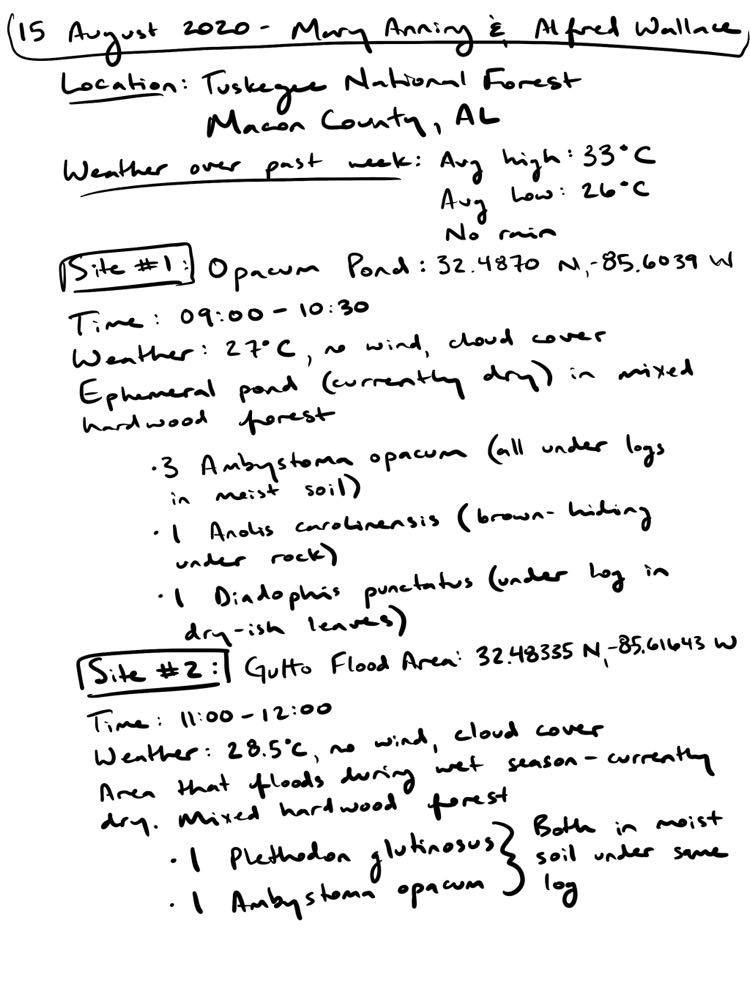
\includegraphics[scale=0.5]{FieldNoteExample.jpg}
  \label{fig:FieldNotes}
\end{figure}


\end{document}% preamble will be ignored
\chapter{\Huge{Exam 1: ``Fishes''}}  \label{SecFish}

% This document is for the Group Meeting Agenda.  The Agenda should
% be distributed to each member (and other invitees) and to the TA
% prior to the meeting (hopefully the day before) so that each member
% will have adequate time to prepare for the meeting.  The best way
% to accomplish the distribution of the agenda is to email the LaTeX
% file to all members and TA.
%
%\documentstyle[fullpage]{article}
\documentclass[a4paper,12pt]{article}
\usepackage{fullpage}
\usepackage{cite}
\usepackage{url}
\usepackage{xcolor}
\usepackage{setspace}
\usepackage[version=4]{mhchem}
\usepackage{upgreek}
\usepackage[margin=0.75in]{geometry}
% For figure:
\usepackage{graphicx}
\usepackage{float}
% For table:
\usepackage{makecell}
\makeatletter
% we use \prefix@<level> only if it is defined
\renewcommand{\@seccntformat}[1]{%
  \ifcsname prefix@#1\endcsname
    \csname prefix@#1\endcsname
  \else
    \csname the#1\endcsname\quad
  \fi}
% define \prefix@section
\newcommand\prefix@section{}
\makeatother
\begin{document}

%
% This section gives the general information about the meeting such
% as the title, who it was called by, when and where the meeting
% will take place, what type of meeting it is (planning, design,
% problem-solving, decision-making, etc.), and of course who is
% invited to attend.
%

\pagestyle{fancyplain}
\fancyhf{}
\lhead{ \fancyplain{}{BIOL 4020 – Vertebrate Biodiversity - Exam 1: ``Fishes''}}
%\chead{ \fancyplain{}{}}
\rhead{ \fancyplain{}{Fall 2020}}
%\rfoot{\fancyplain{}{page \thepage\ of \pageref{LastPage}}}
\fancyfoot[RO, LE] {page \thepage\ of \pageref{LastPage}}
\thispagestyle{plain}

\section*{Evolutionary trees to know:}
\begin{figure}[h]
\centering
  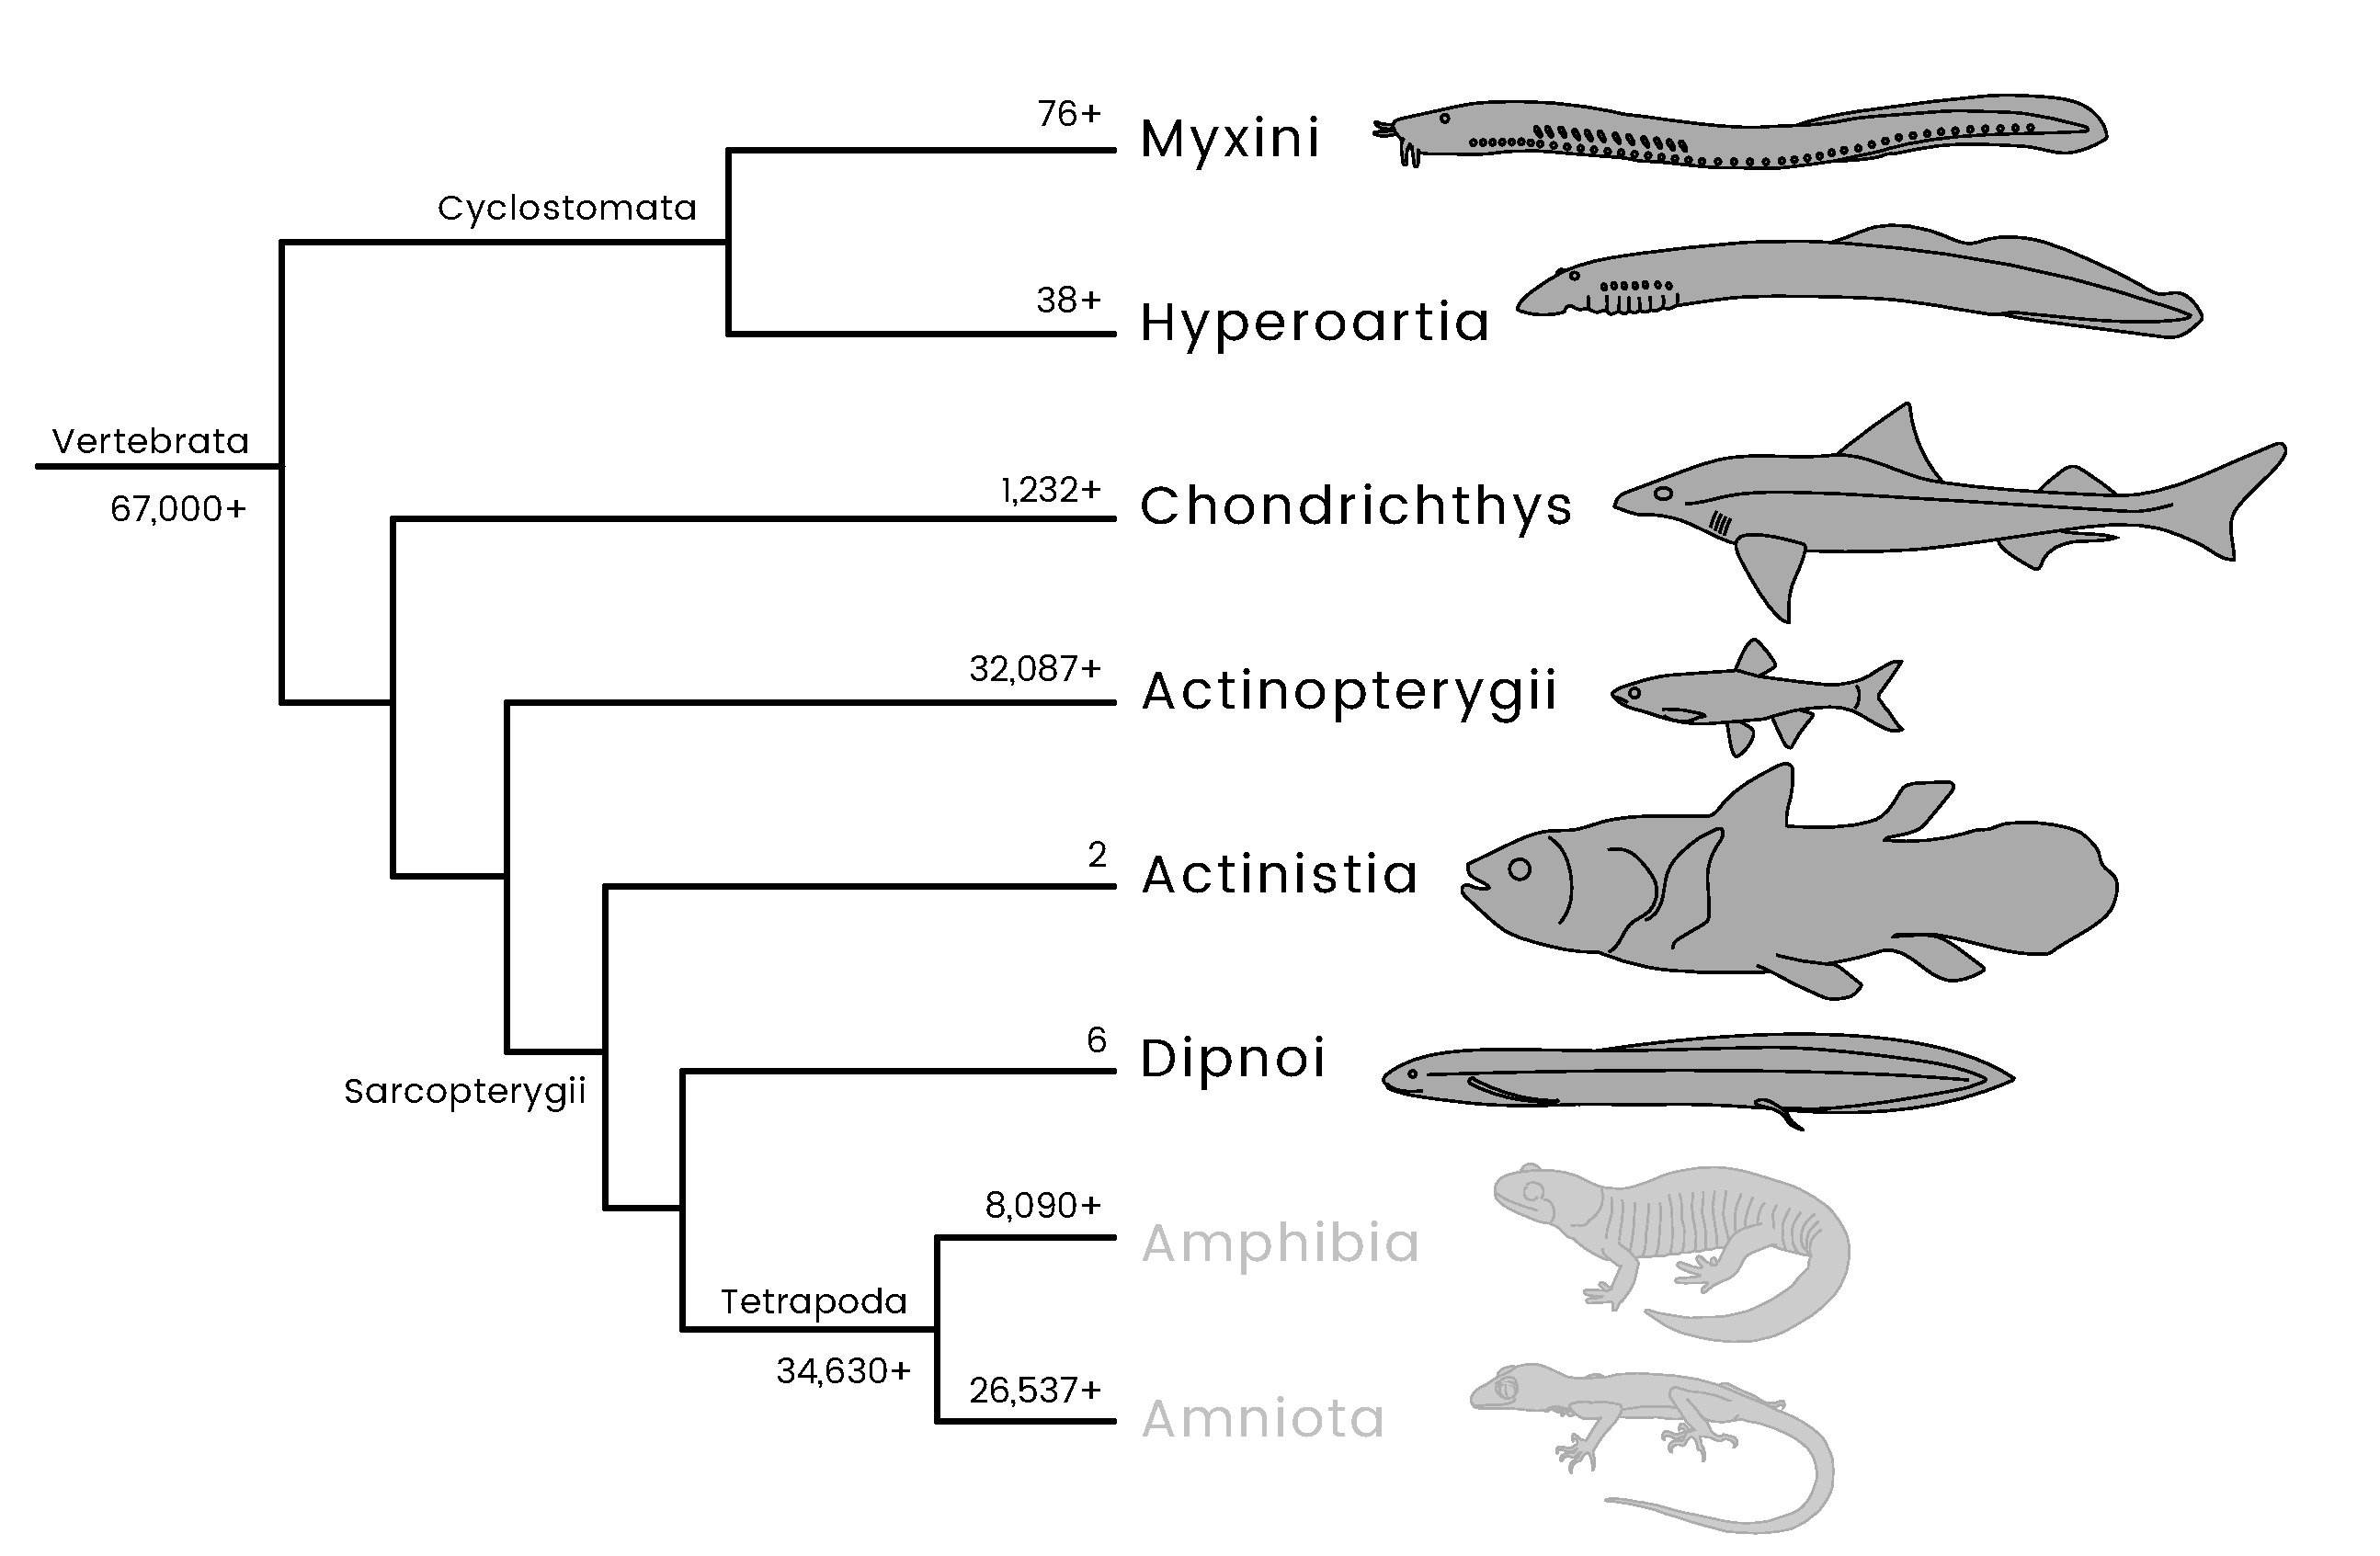
\includegraphics[scale=0.3]{Vertebrata_fishes_tre.pdf}
  \caption{How ``fish'' relate to other vertebrates}
  \label{fig:Fishes}
\end{figure}

\begin{figure}[h]
\centering
  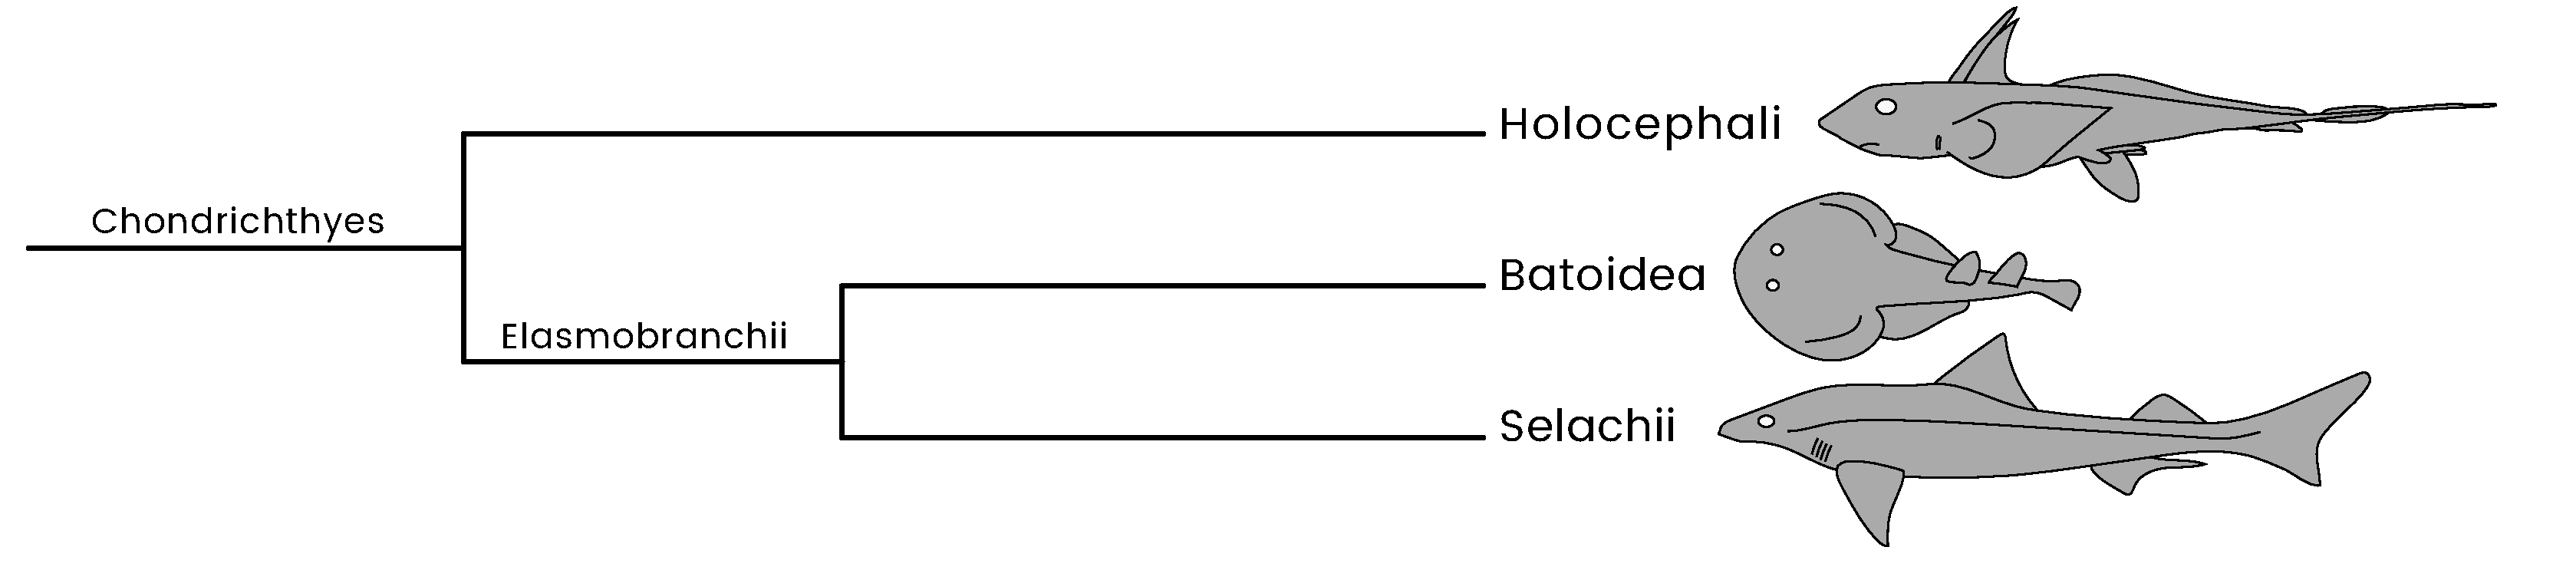
\includegraphics[scale=0.3]{Chondrichthys_tre.pdf}
  \caption{Major groups within Chondrichthys}
  \label{fig:Chondrichthys}
\end{figure}

\begin{figure}[h]
\centering
  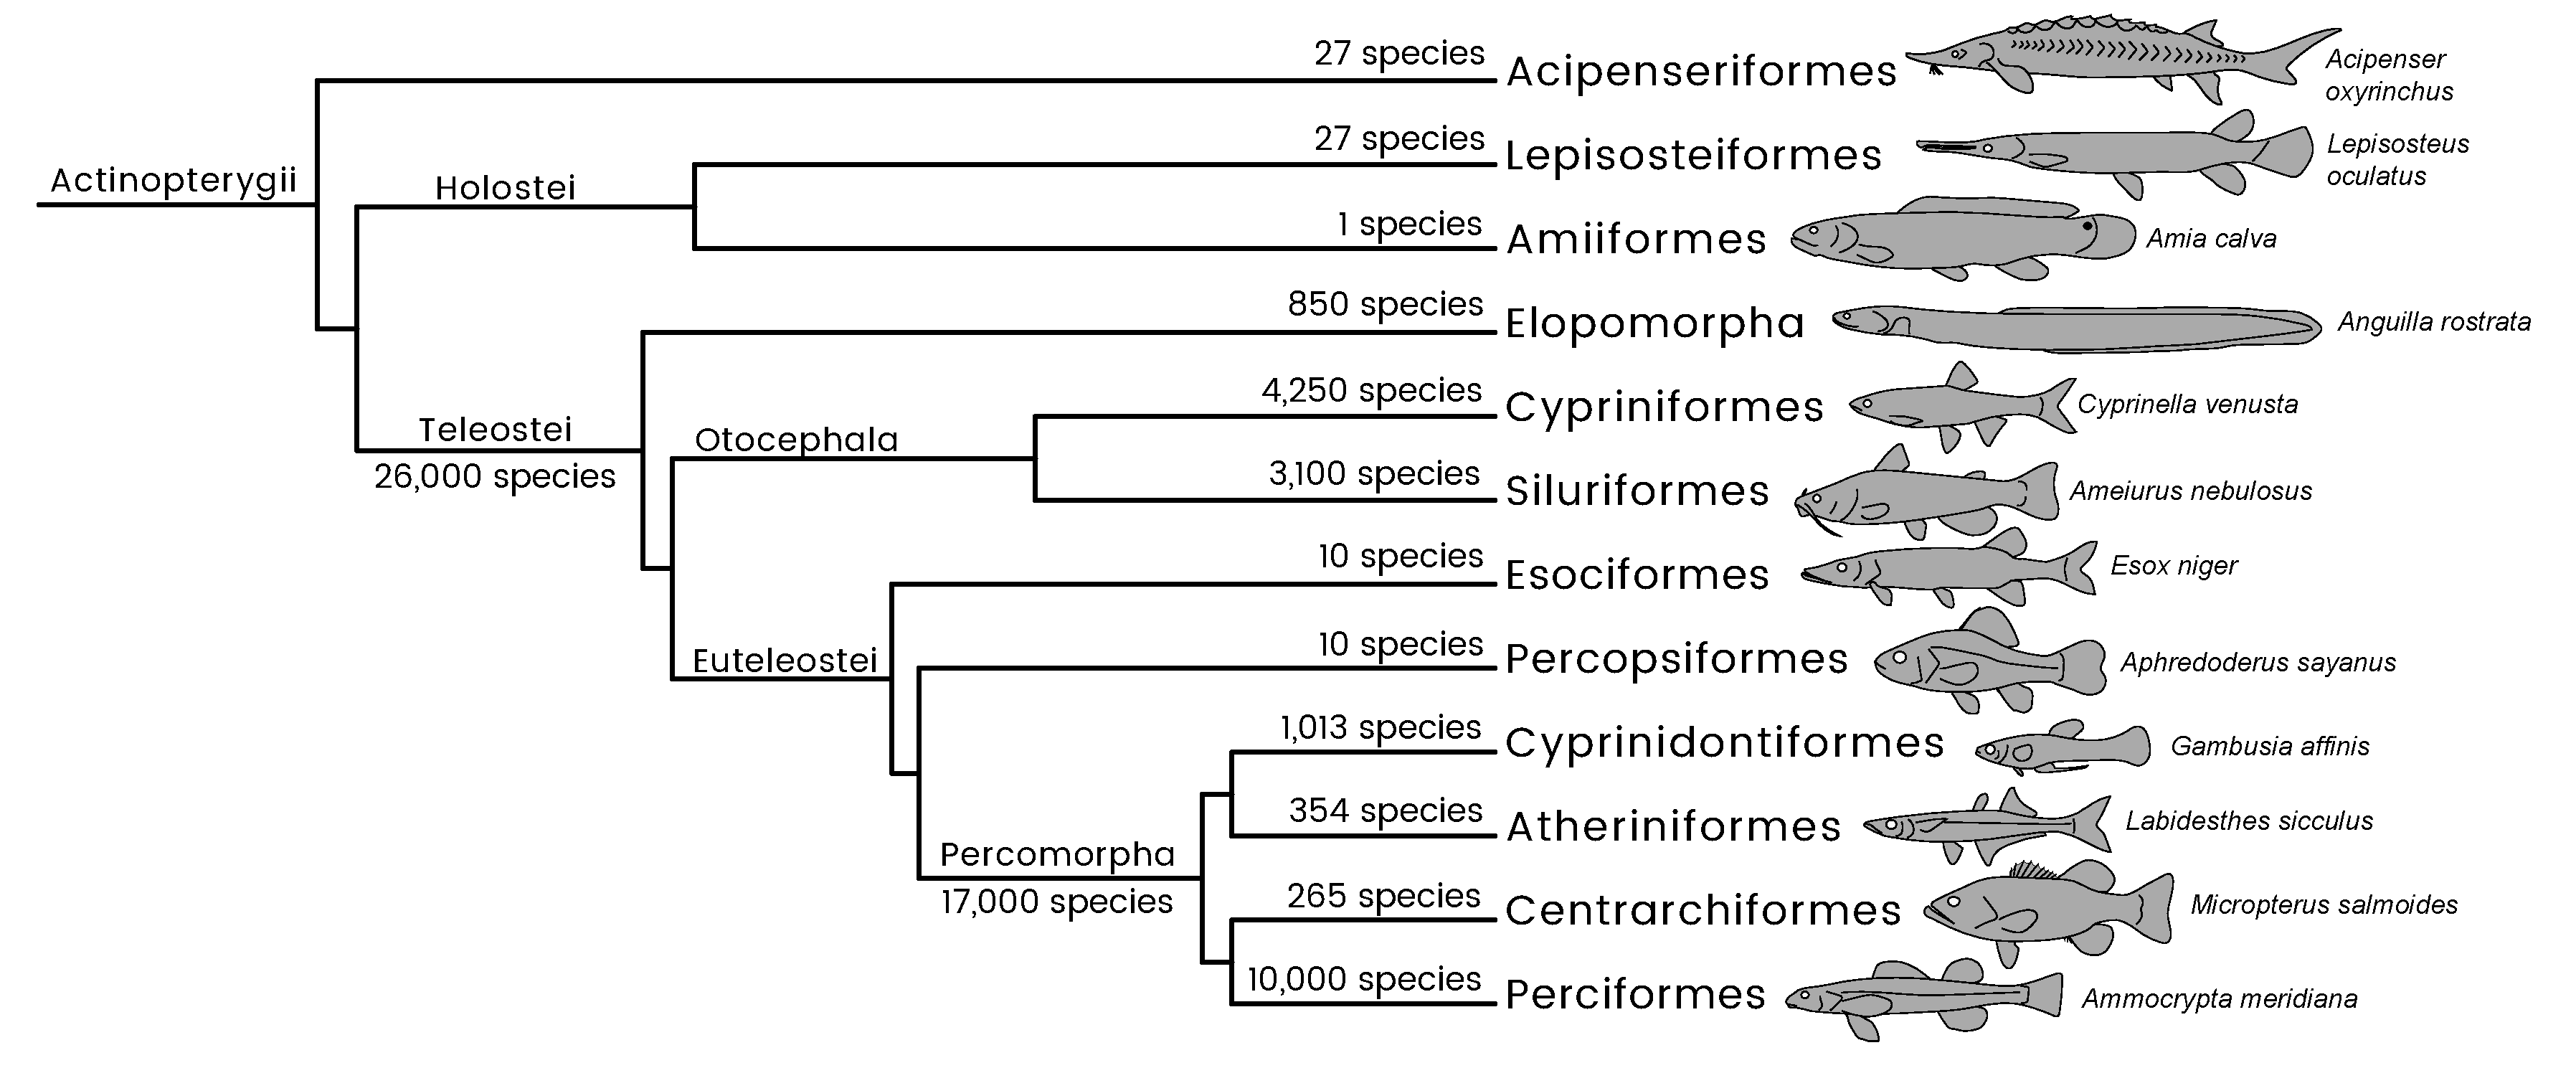
\includegraphics[scale=0.3]{Actinopterygii_tre.pdf}
  \caption{Major groups within Actinopterygii}
  \label{fig:Actinopterygii}
\end{figure}

\begin{singlespace}
\section*{Evolutionary terms to know:}
\begin{itemize}
  \large{
  \item{Monophyly}
  \item{Clade}
  \item{Paraphyly}
  \item{Grade}
  }
\end{itemize}
\end{singlespace}

\begin{figure}[h]
\centering
  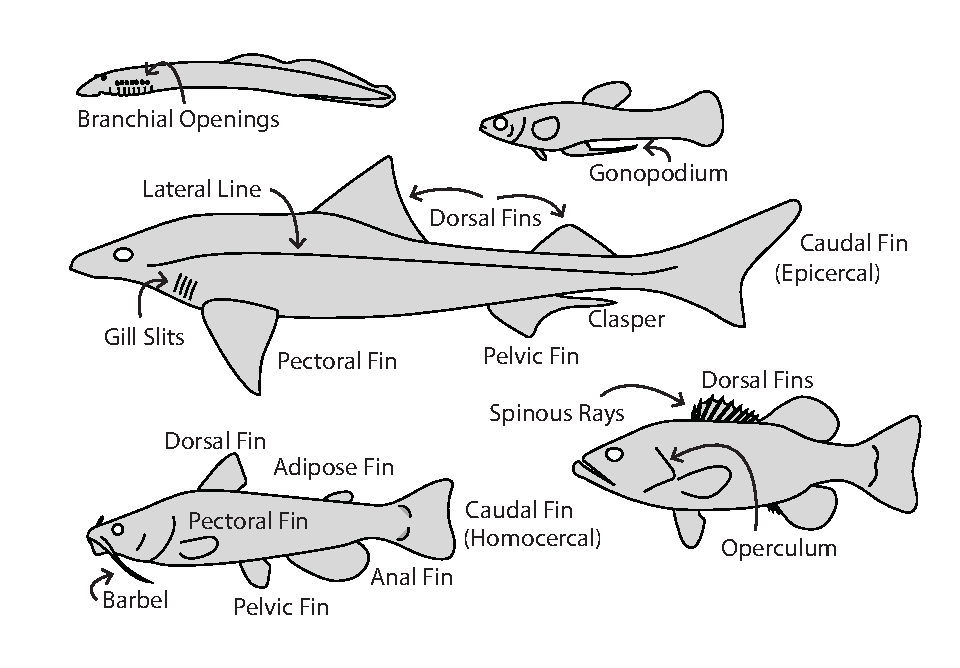
\includegraphics{FishAnatomy.pdf}
  \caption{Fish anatomical terms to know}
  \label{fig:FishAnatomy}
\end{figure}

\section*{Focal taxonomic groups ($\star$ groups you need to be able to photo ID and place in a phylogeny)}
\begin{description}
\item\textbf{Cyclostomata} (jawless fish) \\ No vertebral central, no pectoral / pelvic fins with endoskeletal support, gill openings pores rather than slits, elongated body
\begin{itemize}
  \item{\textbf{Myxini} (hagfish) $\star$}\\ 12 pairs of gill openings, mucous glands lateroventraly along the body, Paired of sensing tentacles
  \item{\textbf{Hyperoartia} (lamprey)$\star$}\\ 7 pairs of gill openings, single mediodorsal nostral, funnel-shaped mouth surrounded by oral disk
\end{itemize}
\item\textbf{Gnathostomata} (jawed fish)
\begin{itemize}
  \item{\textbf{Chondrichthys} (cartilagenous fish; Fig. \ref{fig:Chondrichthys})}$\star$\\ Cartilagenous endoskeleton, placoid scales, no swim bladder
  \begin{itemize}
    \item{\textbf{Holocephali} (Chimaera)$\star$}\\ Operculum over 4 gill arches, teeth are grinding plates, no cloaca (anal and urogenital openings separate)
    \item{\textbf{Elasmobranchii}} \\ Heterocercal tail, internal fertilization via claspers
    \begin{itemize}
      \item{\textbf{Selachii} (Sharks)$\star$}\\ Heterocercal tail, 5-7 exposed lateral gill slits anterior to pectoral fins
      \item{\textbf{Batoidea} (Skates \& Rays)$\star$} \\ Dorsoventrally flattened body, expanded pectoral fins fused to the head
    \end{itemize}
  \end{itemize}
  \item{\textbf{Osteichthyes} (bony fish)} \\ endoskeletons composed (at least partially) of ossified tissue
  \begin{itemize}
    \item{\textbf{Actinopterygii} (ray-finned fish; Fig. \ref{fig:Actinopterygii})}$\star$\\ raylike supports in fins, radial bones of pectoral girdle all attached to the scapulocoracoid complex
    \begin{itemize}
      \item{\textbf{Acipenseriformes}} \\ Heterocercal tail, only dermal bones of head and pectoral girdle ossified
      \begin{itemize}
        \item{\textbf{family ACIPENSERIDAE} (sturgeons)} \\ Robust body armed with 5 longitudinal rows of large bony plates, pronounced snout with 4 sensitive barbels, largest freshwater fish
          \item{\textbf{\textit{   Scaphirhynchus platorynchus}} (shovel-nosed sturgeon)$\star$} \\ highly endangered, 4 lobes on lower lip, fringed barbels on front of mouth
        \item{\textbf{family POLYODONTIDAE} (paddlefish)} \\ paddle/spatula-like snout, virtually naked skin, greatly extended operculum
          \item{\textbf{\textit{   Polyodon spathula}} (American paddlefish)$\star$} \\ grows up to 7 ft, filter-feeder
      \end{itemize}
      \item{\textbf{Lepisosteiformes} (gars)$\star$} \\ elongate jaws with teeth, elongate body with dorsal and anal fins located caudally, abbreviated heterocercal tail, swim bladder can be used for respiration
      \begin{itemize}
        \item{\textbf{\textit{   Lepisosteus oculatus}} (spotted gar)} \\ olive brown to black, spots on body, head, and fins
      \end{itemize}
      \item{\textbf{Amiiformes} (bowfin)} \\ swim bladder can be used for respiration, round snout
      \begin{itemize}
        \item{\textbf{\textit{   Amia calva}} (bowfin)$\star$} \\ body nearly cylindrical, long dorsal fin, abbreviated heterocercal tail, gular plate
      \end{itemize}
      \item{\textbf{Elopomorpha}} \\ Leptocephalus larvae
      \begin{itemize}
        \item{\textbf{Anguilliformes} (eels)} \\ body elongate, lack pelvic fins, pelvic girdle is often absent and when present is remote from skull
        \item{\textbf{\textit{   Anguilla rostrata}} (American eel)$\star$} \\ long anal and dorsal fins
      \end{itemize}
      \item{\textbf{Cypriniformes}$\star$} \\ Kinethmoid bone for jaw protrusion
      \begin{itemize}
        \item{\textbf{family CATOSTOMIDAE} (suckers)} \\ Pelvic fins abdominal, 1 dorsal fin, dorsal fin rays 10 or more, large mouth suckers ventral
        \item{\textbf{\textit{   Carpiodes velifer}} (highfin carpsucker)$\star$} \\ Long sickle-shaped dorsal fin, projection on lower lip
        \item{\textbf{\textit{   Hypentelium etowanum}} (Alabama hogsucker)} \\ Cylindrical body, very pronounced ventral sucker, top of head between eyes flat or concave
        \item{\textbf{family CYPRINIDAE} (minnows and carp)} \\ no teeth on jaws, modified teeth on gill arches, fin rays soft and flexible, pelvic fins abdominal
        \item{\textbf{\textit{   Cyprinella venusta}} (black-tail shiner)$\star$} \\ large black spot at base of caudal fin
        \item{\textbf{\textit{   Pimephales vigilax}} (bullhead minnow)} \\ blunt snout, leading ray stout and detached from first principle ray, light tail spot
        \item{\textbf{\textit{   Notropis ammophilus}} (orangefin shiner)} \\ 8 dorsal rays, prominant orange fins
      \end{itemize}
      \item{\textbf{Siluriformes} (catfish)$\star$} \\ Single spinous ray at beginning of dorsal and pectoral fins, adipose fin, pectoral girdle modified to form locking mechanism for pectoral fin spine
      \begin{itemize}
        \item{\textbf{\textit{   Ictalurus punctatus}} (channel catfish)} \\ caudal fin forked, 9 pelvic rays, deeply forked tail
        \item{\textbf{\textit{   Ameiurus nebulosus}} (brown bullhead)$\star$} \\ 8 pelvic rays, caudal fin not deeply forked, white or yellow chin barbels
      \end{itemize}
      \item{\textbf{Esociformes}} \\ Elongate body, tootless maxilla, posterior dorsal and anal fins
      \begin{itemize}
        \item{\textbf{\textit{   Esox niger}} (chain pickerel)$\star$} \\ duckbill-like snout, snout longer than postorbital length of head, abdominal pectoral fins
      \end{itemize}
      \item{\textbf{Percopsiformes}} \\ ctenoid scales, spines on medial fins reduced or lost
      \begin{itemize}
        \item{\textbf{\textit{   Aphredoderus sayanus}$\star$} (pirate perch)} \\ anus anterior between pectoral fins in adults (not in juveniles)
      \end{itemize} 
      \item{\textbf{Cyprinidontiformes}$\star$} \\ unlobed caudal fin, low-set pectoral fins
      \begin{itemize}
        \item{\textbf{family POECILIIDAE} (live-bearers)} \\ small fins, caudal fin rounded, mouth small and directed upward, males have anal fin displaced forward with gonopodium formed from 3 anal rays, elaborate reproductive strategy
        \item{\textbf{\textit{   Gambusia affinis}} (western mosquito fish)$\star$} \\ 6 dorsal fin rays
        \item{\textbf{family FUNDULIDAE} (killifish)} \\ elongate body somewhat laterally compressed with head dorsoventrally flattened, mouth small and turned upward, lower jaw extends beyond upper
        \item{\textbf{\textit{   Fundulus olivaceus}} (black-spotted topminnow)$\star$} \\ Dorsal fin origin posterior from anal fin origin, prominant black stripe with dorsal spotting
      \end{itemize}
      \item{\textbf{Atheriniformes} (silversides)} \\ 2 dorsal fins well separated (first with weak spines), anal fin longer than second dorsal fin, elongate and slightly compressed body
      \begin{itemize}
        \item{\textbf{\textit{   Labidesthes sticculus}} (brook sliverside)$\star$} \\ origin of first dorsal fin near origin of anal fin
      \end{itemize}
      \item{\textbf{Centrarchiformes}$\star$} \\ 2 dorsal fins, 3 or more spines on anal tail, siny dorsal fin confluent with soft dorsal fin
      \begin{itemize}
        \item{\textbf{\textit{   Lepomis cyanellus}} (green sunfish)$\star$} \\ maxilla reaches beneath eye, pectoral fin short and rounded
        \item{\textbf{\textit{   Micropterus salmoides}} (largemouth bass)$\star$} \\ large mouth with lower jaw projecting, smaller spiny dorsal fin separated by notch from the second dorsal fin
      \end{itemize}
      \item{\textbf{Perciformes}$\star$} \\ spines in dorsal and anal fins
      \begin{itemize}
        \item{\textbf{family COTTIDAE} (sculpins)} \\ skin mostly naked, high eyes directed upward, body robust with large head
        \item{\textbf{\textit{   Cottus carolinae}} (banded sculpin)} \\ mottled brown with dark vertical banding, broad head, body narrows caudally
        \item{\textbf{family PERCIDAE} (perches and darters)} \\ two dorsal fins, dorsal fins separated bya  space, 2 anal spines
        \item{\textbf{\textit{   Ammocrypta meridiana}} (southern darter)$\star$} \\ elongate body, blunt snout, caudal fin truncate
      \end{itemize}
    \end{itemize}
    \item{\textbf{Sarcopterygii}$\star$} \\ radial bones of pectoral girdle not all attached to the scapulocoracoid complex
    \begin{itemize}
      \item{\textbf{Actinistia} (lobe-finned fish)$\star$} \\ skull divided anteriorly and posteriorly, widely distributed 400 million years ago
      \item{\textbf{Dipnoi} (lung fish)$\star$} \\ elongated and laterally compressed body, respire by gills and lungs
    \end{itemize}
  \end{itemize}
\end{itemize}
\end{description}

\end{document}
% preamble will be ignored
\chapter{\Huge{Exam 2: Amphibians}} \label{SecAmphib}

% This document is for the Group Meeting Agenda.  The Agenda should
% be distributed to each member (and other invitees) and to the TA
% prior to the meeting (hopefully the day before) so that each member
% will have adequate time to prepare for the meeting.  The best way
% to accomplish the distribution of the agenda is to email the LaTeX
% file to all members and TA.
%
%\documentstyle[fullpage]{article}
\documentclass[a4paper,12pt]{article}
\usepackage{fullpage}
\usepackage{cite}
\usepackage{url}
\usepackage{xcolor}
\usepackage{setspace}
\usepackage[version=4]{mhchem}
\usepackage{upgreek}
\usepackage[margin=0.75in]{geometry}
% For figure:
\usepackage{graphicx}
\usepackage{float}
% For table:
\usepackage{makecell}
\makeatletter
% we use \prefix@<level> only if it is defined
\renewcommand{\@seccntformat}[1]{%
  \ifcsname prefix@#1\endcsname
    \csname prefix@#1\endcsname
  \else
    \csname the#1\endcsname\quad
  \fi}
% define \prefix@section
\newcommand\prefix@section{}
\makeatother
\begin{document}

%
% This section gives the general information about the meeting such
% as the title, who it was called by, when and where the meeting
% will take place, what type of meeting it is (planning, design,
% problem-solving, decision-making, etc.), and of course who is
% invited to attend.
%

\pagestyle{fancyplain}
\fancyhf{}
\lhead{ \fancyplain{}{BIOL 4020 – Vertebrate Biodiversity - Exam 2: Amphibians}}
%\chead{ \fancyplain{}{}}
\rhead{ \fancyplain{}{Fall 2020}}
%\rfoot{\fancyplain{}{page \thepage\ of \pageref{LastPage}}}
\fancyfoot[RO, LE] {page \thepage\ of \pageref{LastPage}}
\thispagestyle{plain}

\begin{figure}[h]
\centering
  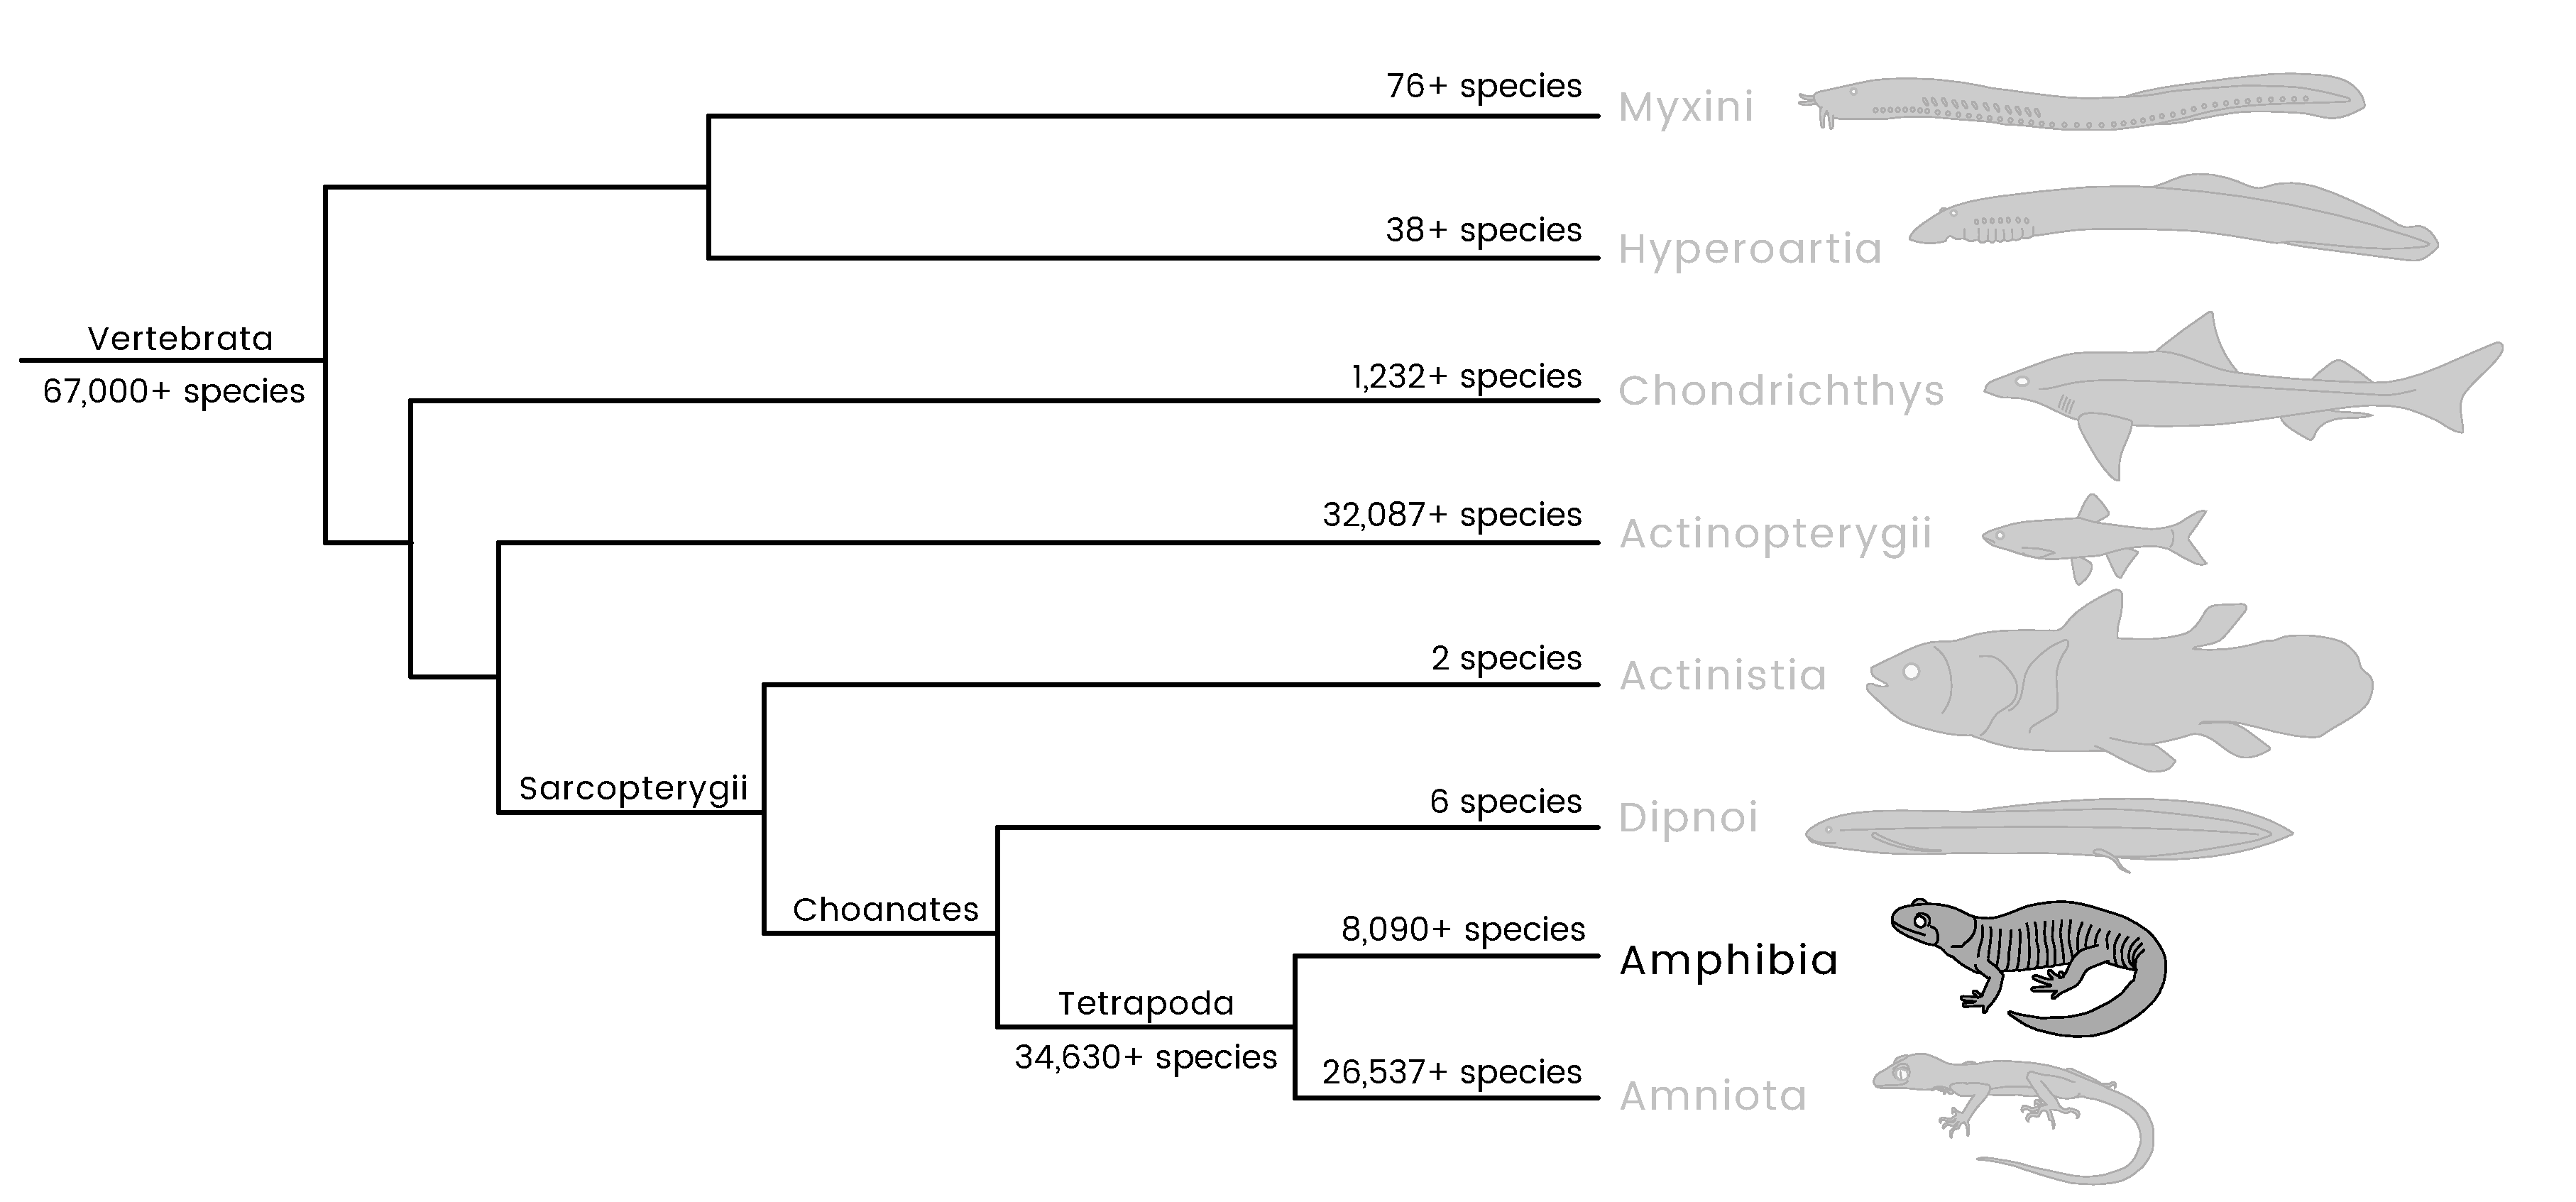
\includegraphics[scale=0.3]{Vertebrata_amphib_tre.pdf}
  \caption{Amphibian placement within Vertebrata}
  \label{fig:Vertebrates2}
\end{figure}

\begin{figure}[h]
\centering
  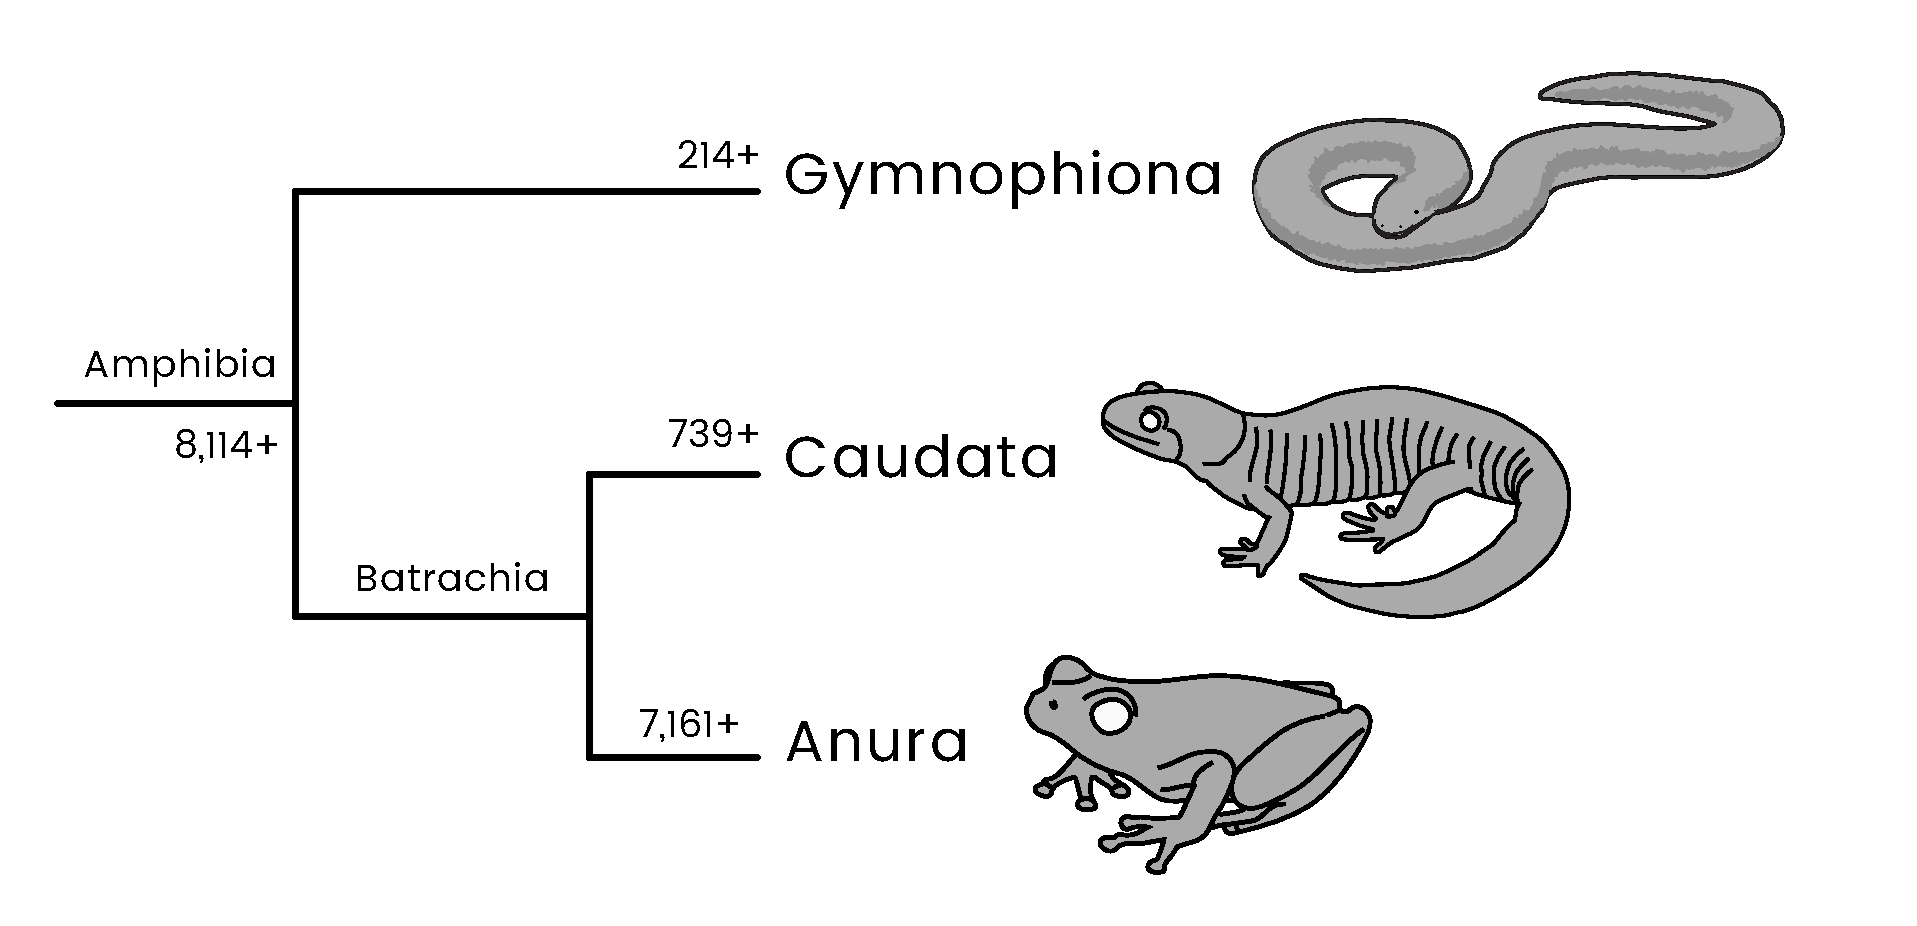
\includegraphics[scale=0.3]{Amphibia_tre.pdf}
  \caption{Amphibian Relationships}
  \label{fig:Amphibia}
\end{figure}

\begin{figure}[h]
\centering
  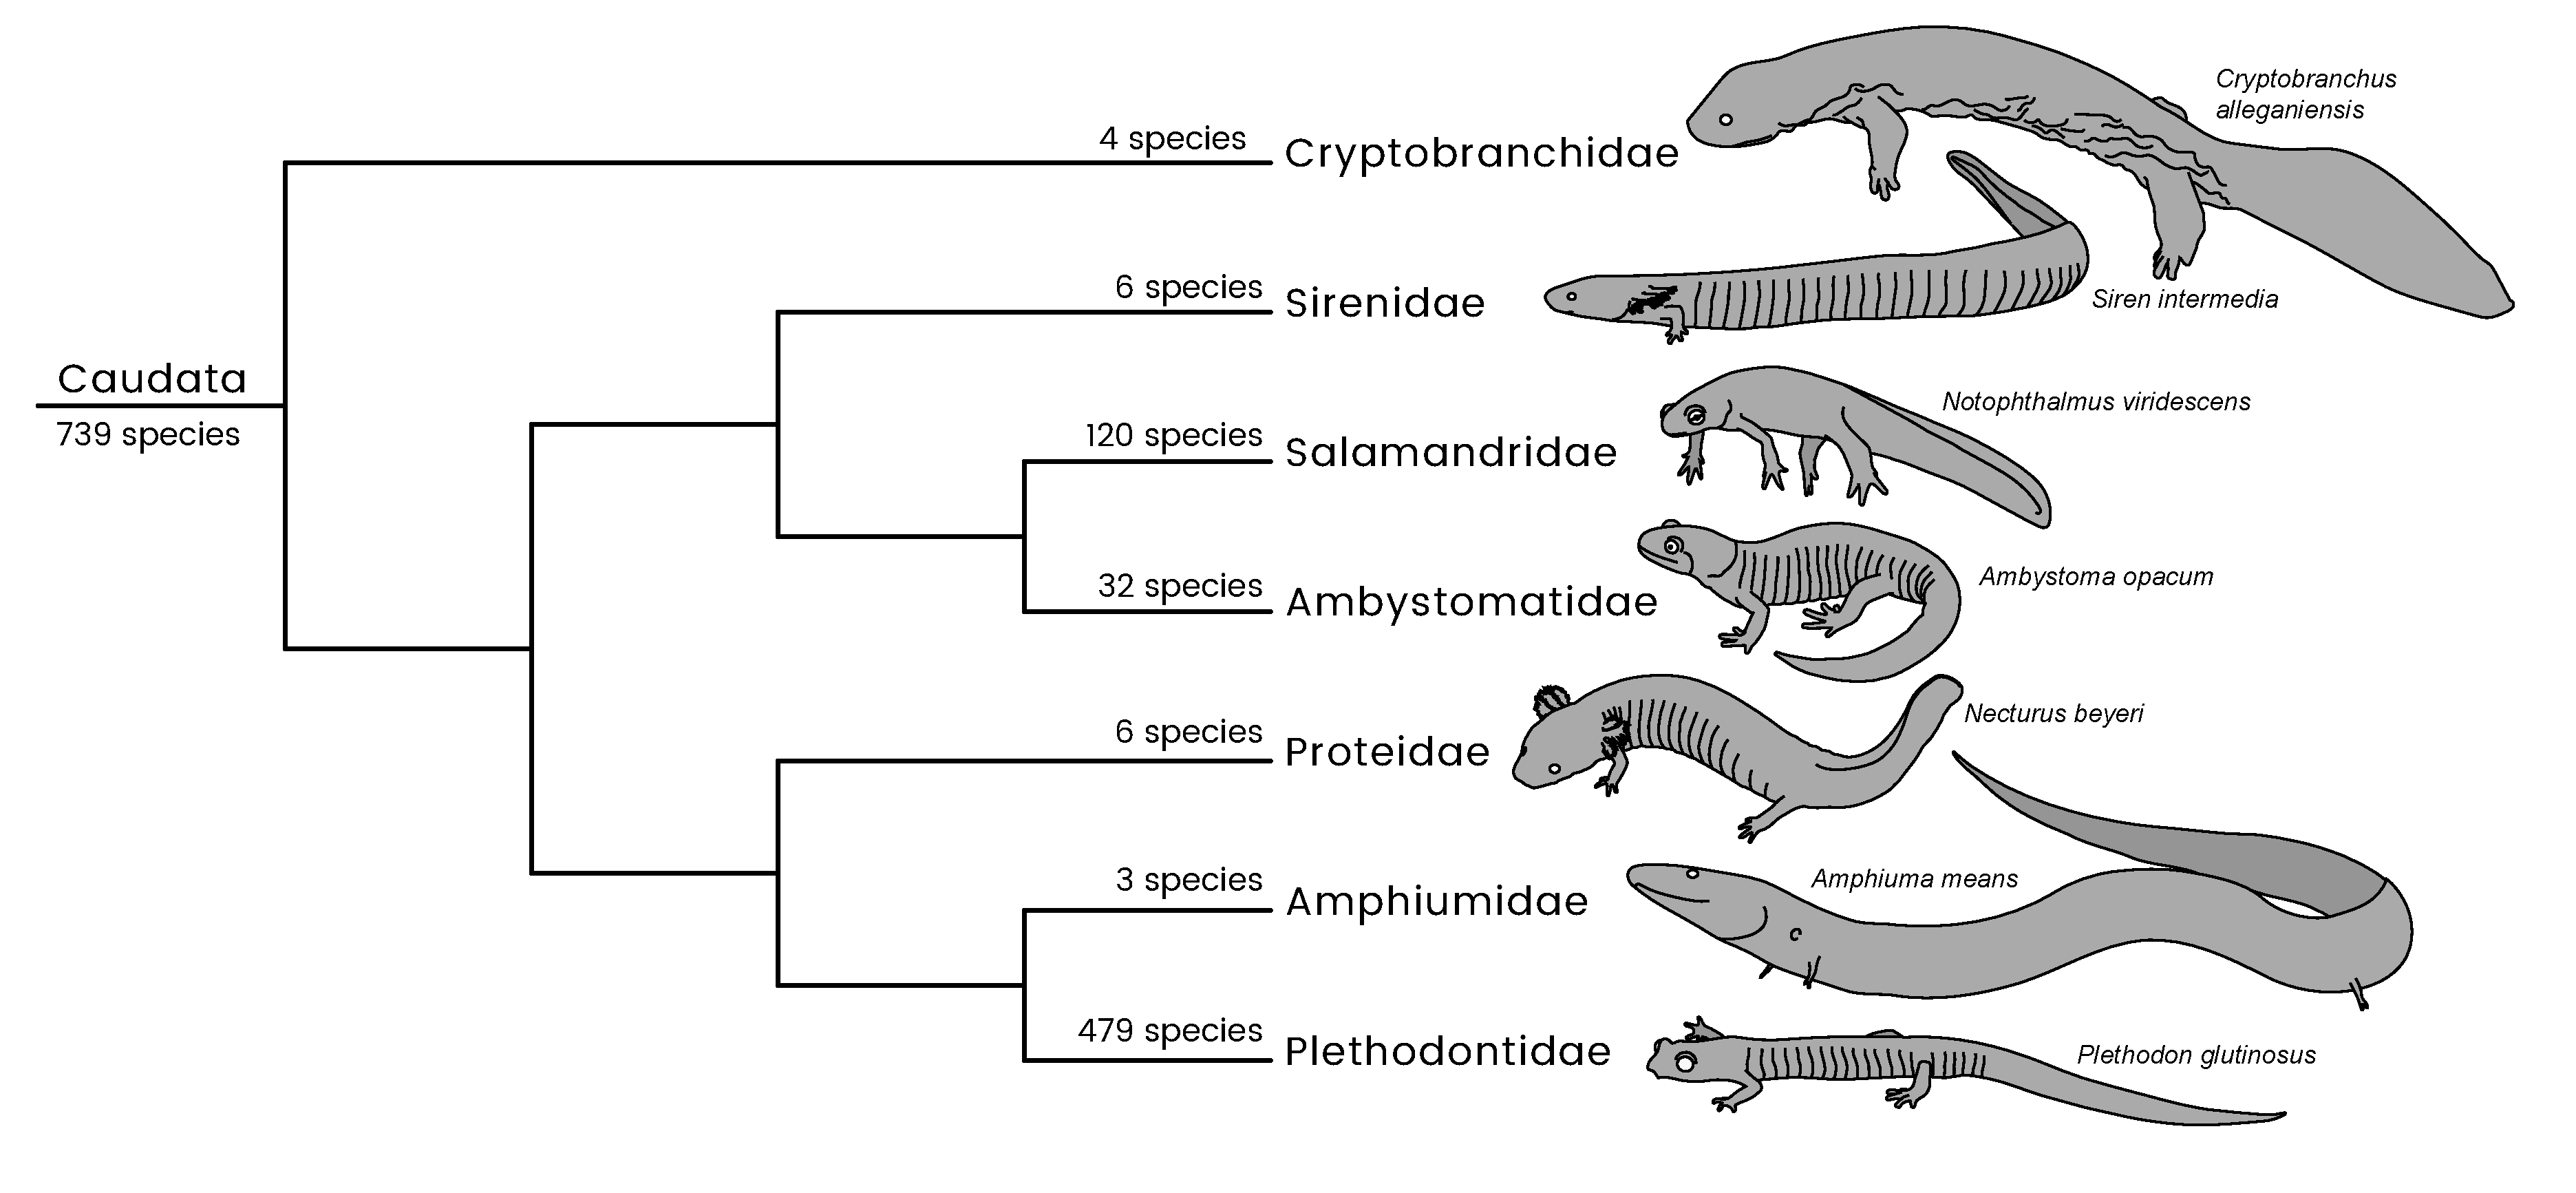
\includegraphics[scale=0.3]{Caudata_tre.pdf}
  \caption{Caudata Relationships (abbreviated)}
  \label{fig:Caudata}
\end{figure}

\begin{figure}[h]
\centering
  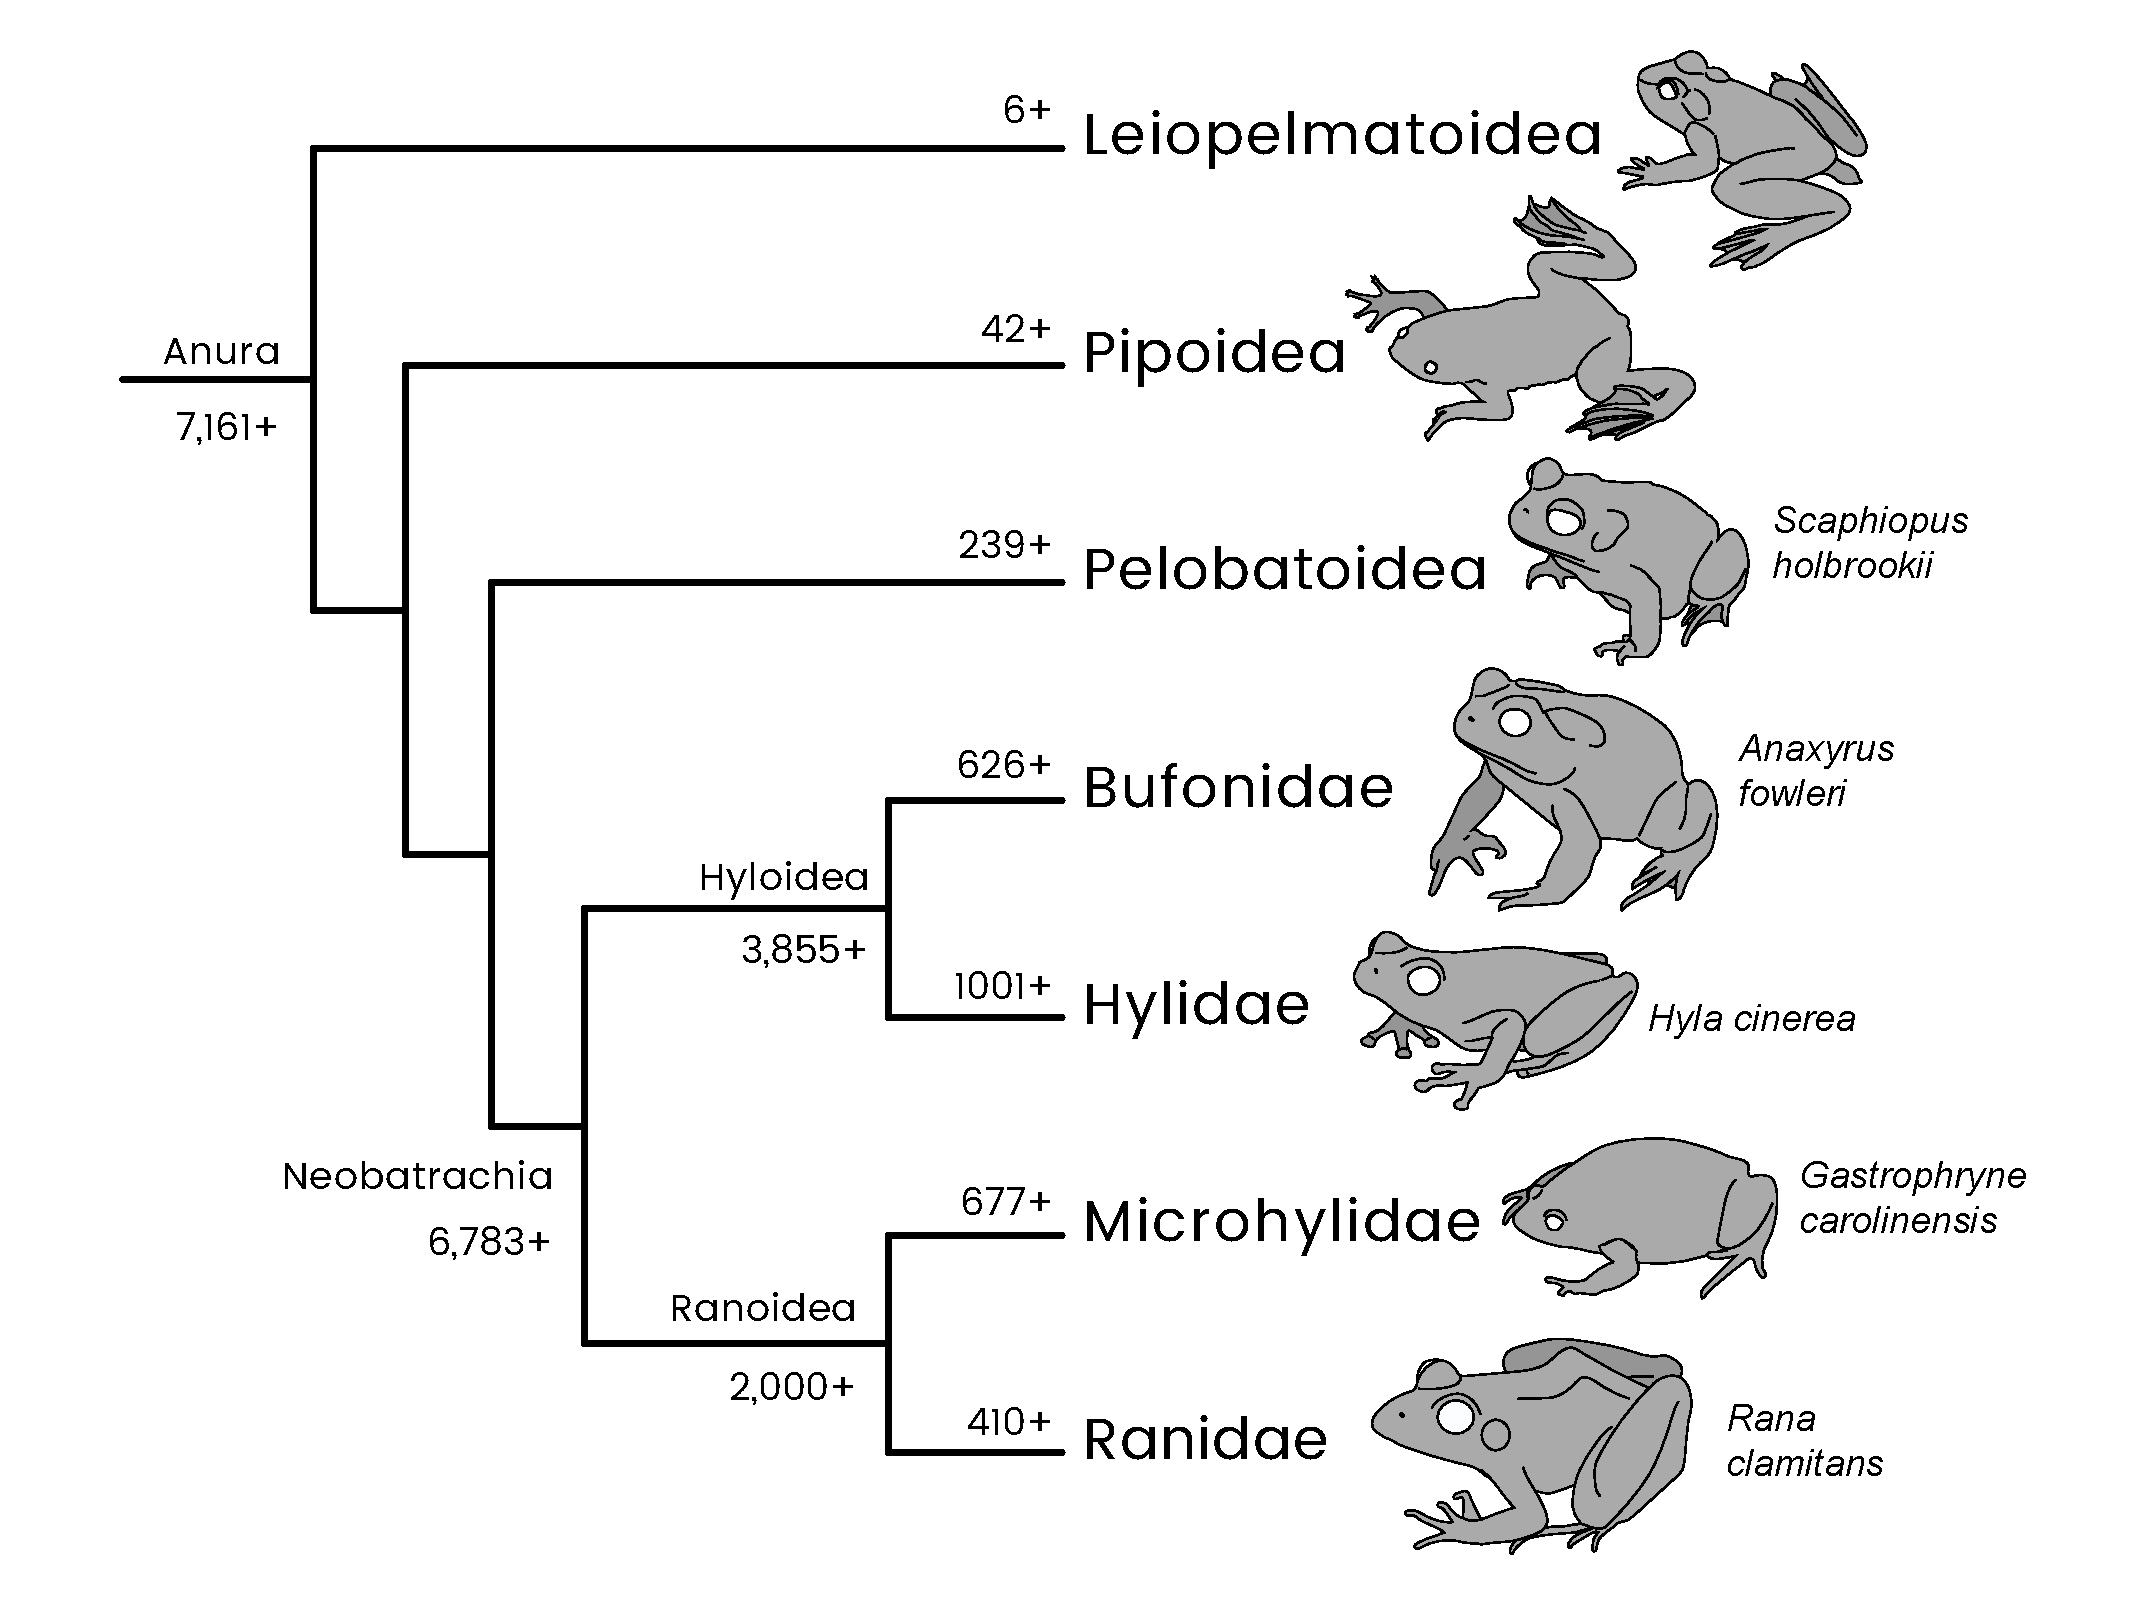
\includegraphics[scale=0.3]{Anura_tre.pdf}
  \caption{Anura Relationships (abbreviated)}
  \label{fig:Anura}
\end{figure}

\begin{figure}[h]
\centering
  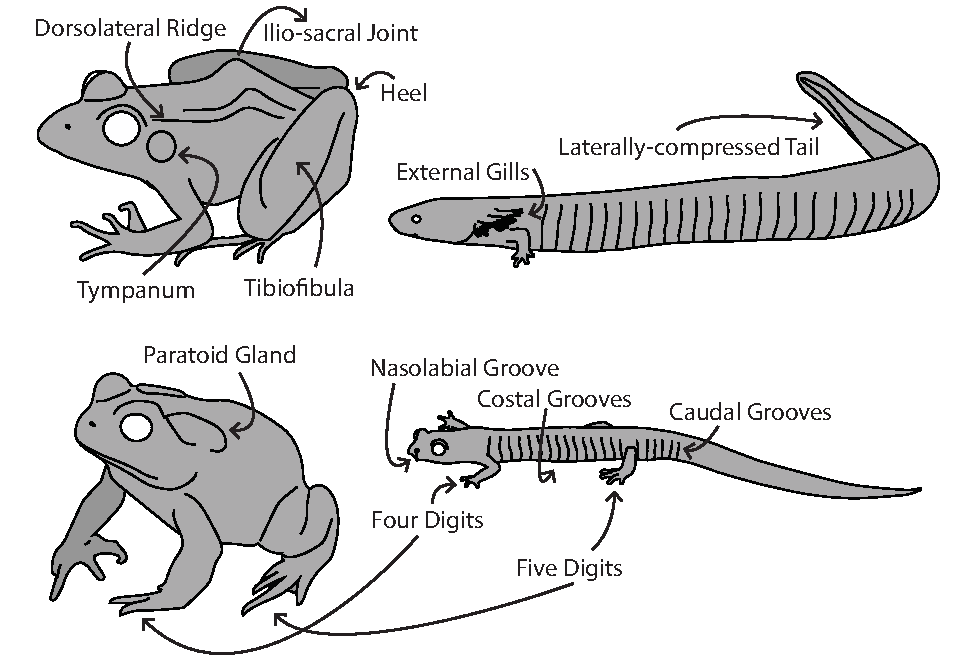
\includegraphics{AmphibianAnatomy.pdf}
  \caption{Amphibian anatomical terms to know}
  \label{fig:Anura}
\end{figure}

\section*{Focal taxonomic groups ($\star$ groups you need to be able to photo ID and place in a phylogeny. $\mathsection$ denotes species for which you need to audio ID calls.)}
\begin{description}
\item{\textbf{Gymnophiona} (caecilians) $\star$} \\ No limbs, cylindrical body, tail short or absent, cloaca towards end of body, strong skull with pointed snout, pair of tentacles between eyes and mouth (olfactory), bodies distinctly segmented by annuli (each segment contains a single vertebra)
\item{\textbf{Caudata} (salamanders) $\star$} \\ tailed, body not globular
\begin{itemize}
  \item{\textbf{family CHRYPTOBRANCHIDAE} (giant salamanders) $\star$} \\ largest living salamanders, stout bodies, four short and well-developed limbs, laterally compressed tail, single pair of gill slits
  \begin{itemize}
    \item{\textbf{\textit{   Chryptobranchus alleganiensis}} (American hellbender) $\star$} \\ Flat head, fringe of skin along sides of body, external gill openings but no visible gills, reduced eyes
  \end{itemize}
  \item{\textbf{family SIRENIDAE} (sirens) $\star$} \\ No hind limbs, external gills
  \begin{itemize}
    \item{\textbf{\textit{   Siren intermedia}} (lesser siren)} \\ Less than 36 costal grooves
  \end{itemize}  
  \item{\textbf{family SALAMANDRIDAE} (newts and European salamanders)} \\ Four limbs, no gill openings, no nasolabial groove, ridge down middorsum, no costal grooves (or costal grooves above ribs), rough skin
  \begin{itemize}
    \item{\textbf{\textit{   Notophthalmus viridescens} $\star$} (Eastern newt)} \\ Adult stage: olive / yellow ground color, spotted (red spots in reproductively active males); Eft stage: red or orange ground color with red spots
  \end{itemize}
  \item{\textbf{family AMBYSTOMATIDAE} (mole salamanders) $\star$} \\ Costal grooves present, dorsum round and lacking ridge, no nasolabial grooves, heavy bodied, heavy tailed, lack gills and gill slits and have moveable eyelids
  \begin{itemize}
    \item{\textbf{\textit{   Ambystoma opacum}} (marbled salamander) $\star$} \\ black ground color with white/silvery crossbands on dorsum (some of which are ocassionally broken- more pronounced in males)
    \item{\textbf{\textit{   Ambystoma maculatum}} (spotted salamander) $\star$} \\ black ground color with orange/yellow dorsal spots or blotches
    \item{\textbf{\textit{   Ambystoma mexicanum}} (axolotl)} \\ larval traits retained (no moveable eyelinds, external gills), model organism
  \end{itemize}
  \item{\textbf{family PROTEIDAE} (water dogs) $\star$} \\ External gills, four well-developed limbs, moderately robust body, laterally compressed tails
  \begin{itemize}
    \item{\textbf{\textit{   Necturus beyeri}} (Gulf Coast waterdog)} \\ cylindrical body, four toes on front and hind limbs, spotted body (light spotting in adults)
  \end{itemize}
  \item{\textbf{family AMPHIUMIDAE} (congo eels) $\star$} \\ External gill slits, four reduced limbs (with 3 or fewer toes)
  \begin{itemize}
    \item{\textbf{\textit{   Amphiuma means}} (two-toed amphiuma)} \\ 2 toes on each limb
  \end{itemize}
  \item{\textbf{family PLETHODONTIDAE} (lungless salamanders) $\star$} \\ Nasolabial grooves, four well-developed limbs with 4-5 toes, no ridge down mid-dorsum, slim body
  \begin{itemize}
    \item{\textbf{\textit{   Phaeognathus hubrichti}} (Red Hills salamander)} \\ large, plain brown, 20-22 costal grooves
    \item{\textbf{genus\textit{   Desmognathus}} (dusky salamanders) $\star$} \\ face with light stripe from eye to angle of jaw
    \item{\textbf{genus\textit{   Eurycea}} (brook salamanders)} \\ lacking canthus rostralis, less than 15 costal grooves, laterally compressed or keeled tail, venter without markings, face without lights stripe from eye to angle of jaw
    \begin{itemize}
      \item{\textbf{\textit{   Eurycea cirrigera}} (two-lined salamander)} \\ yellowish to orange-brown dorsum with dark dorsolateral stripe from snout to near tail tip
      \item{\textbf{\textit{   Eurycea guttolineata}} (three-lined salamander)} \\ yellowish to orange-brown dorsum with dorsolateral and mid-dorsal black stripe
    \end{itemize}
    \item{\textbf{genus\textit{   Plethodon}} (woodland salamanders)} \\ body not as elongate as \textit{Phaeognathus}, tips of digits lacking expanded disks, Tail not keeled venter without conspicuous markings
    \begin{itemize}
      \item{\textbf{\textit{   Plethodon glutinosus} $\star$} (Southern slimy slamander)} \\ ground color brown to black with light spots or flecks
    \end{itemize}  
    \item{\textbf{genus\textit{   Pseudotriton}}} \\ body relatively stout, costal grooves 16-18, lacking canthus rostralis
    \begin{itemize}
      \item{\textbf{\textit{   Pseudotriton ruber}} (red salamander)} \\ ground color brown to black with light spots or flecks
    \end{itemize}
  \end{itemize}
\end{itemize}
\item\textbf{Anura} (frogs) \\ tailless with globular body
\begin{itemize}
  \item{\textbf{Leiopelmatoidea}}
  \begin{itemize}
    \item{\textbf{genus\textit{   Ascaphus}} (Tailed frog) $\star$} \\ modification of cloaca and tail muscles produces intromittent or copulatory organ in males
  \end{itemize}
  \item{\textbf{Pipoidea}}
  \begin{itemize}
    \item{\textbf{family PIPIDAE}} \\ dorsoventrally depresed bodies and large muscular hindlimbs with webbed feet
    \begin{itemize}
      \item{\textbf{\textit{   Pipa pipa}} (Suriname toad)} \\ extreme dorsoventral compression with squared head, females carry eggs and developing tadpoles on their backs
      \item{\textbf{\textit{   Xenopus laevis}} (African clawed frog)} \\ somewhat egg-shaped body, fully webbed toes, three toes on each foot have conspicuous black claws
    \end{itemize}
  \end{itemize}
  \item{\textbf{Pelobatoidea}}
  \begin{itemize}
    \item{\textbf{family SCAPHIOPODIDAE} (spadefoot toads)} \\ squat body, warty (but soft) skin, large keratinous-edged crescent-shaped tubercle on outer edge of eat hind foot, webbed hind feet
    \begin{itemize}
      \item{\textbf{\textit{   Scaphiopus holbrooki}} (Eastern spadefoot) $\star$ $\mathsection$} \\ vertically elliptical pupils, absent or indistinct paratoid glands
    \end{itemize}
  \end{itemize}
  \item{\textbf{family BUFONIDAE} (true toads) $\star$} \\ squat body, short hind limbs, enlarged toepads, 2 spade-like tubercles on hind feet, round pupil, pronounced paratoid glands, skin dry and warty, throats of males usually dark
  \begin{itemize}
      \item{\textbf{\textit{   Anaxyrus fowleri}} (Fowler's toad) $\star$ $\mathsection$} \\ Paratoid gland touches postorbital ridge, three or more warts in each of largest spots, common "backyard" toad
  \end{itemize}
  \item{\textbf{familiy HYLIDAE} (tree frogs and allies)} \\ long hind limbs, usually enlarged toepads
  \begin{itemize}
    \item{\textbf{genus\textit{   Acris}} (cricket frogs) $\star$ $\mathsection$} \\ Rear of thigh with one or two longitudinal stripes, front of snout with lighvertical lines, hind webbing half-way along fourth toe
    \item{\textbf{genus\textit{   Hyla}}} \\ Hind webbing half-way along fourth toe, greatly expanded toe disks
    \begin{itemize}
      \item{\textbf{\textit{   Hyla cinerea}} (green tree frog) $\star$ $\mathsection$} \\ bright green with white/yellow lateral racing stripe
      \item{\textbf{\textit{   Hyla avivoca}} (bird-voiced tree frog) $\star$ $\mathsection$} \\ coloration variable (gray to green), back of thigh pale yellow to greenskin of dorsum smooth to slightly papillate or pustulate
    \end{itemize}
    \item{\textbf{genus\textit{   Pseudacris}} (chorus frogs)} \\ No webbing on hind toes, tips of digits expanded
    \begin{itemize}
      \item{\textbf{\textit{   Pseudacris crucifer}} (spring peeper) $\star$ $\mathsection$} \\ distinct x pattern on dorsum, small toe pads
    \end{itemize}
  \end{itemize}
  \item{\textbf{familiy RANIDAE} (true frogs) $\star$} \\ No toe pads, extensive toe webbing, expanded tympanic membrane
  \begin{itemize}
    \item{\textbf{\textit{   Rana catesbeianus}} (American bullfrog) $\star$ $\mathsection$} \\ Tympanic membrane larger than eye, no dorsal-lateral ridge (ridge ends at tympanum), largest frog in North America
    \item{\textbf{\textit{   Rana sphenocephalus}} (Southern leopard frog) $\star$ $\mathsection$} \\ Dorsal-lateral ridge reaches groin, rounded dark spots on dorsum, pointed snout
    \item{\textbf{\textit{   Rana clamitans}} (bronze frog) $\star$ $\mathsection$} \\ Dorsal-lateral ridge doesn't reach groin, tympanum same size as eye
  \end{itemize}
  \item{\textbf{familiy MICROHYLIDAE} (narrow-mouth frogs) $\star$} \\ supradigital scutes. Members of this family have lipophilic alkaloids (derived from ant diet) that can be highly toxic $\star$note: this family isn't on the tree, but is nested within \textbf{Hyloidea}
  \begin{itemize}
    \item{\textbf{\textit{   Gastrophryne carolinensis}} (narrow-mouth toad) $\star$ $\mathsection$} \\ Small, tiny head with pointed snout, no webbing between digits
  \end{itemize}\end{itemize}
\end{description}

\end{document}
% preamble will be ignored
\end{document}